% Compiles the paper's result figures on their own: tectonic standalone.tex (or pdflatex).
\documentclass{article}
\usepackage[T1]{fontenc}
\usepackage{times}
\usepackage[margin=1in]{geometry}
\usepackage{graphicx,xcolor,pgfplots}
\usepgfplotslibrary{groupplots,fillbetween}
\pgfplotsset{compat=1.18}
% Shared vector-diagram palette; also used by standalone preview builds.
\usetikzlibrary{arrows.meta,calc}
\definecolor{diagramink}{HTML}{253545}
\definecolor{diagrammuted}{HTML}{60717D}
\definecolor{diagramline}{HTML}{CBD4DA}
\definecolor{diagramlight}{HTML}{F3F6F8}
\definecolor{sparsecolor}{HTML}{8B8FCA}
\definecolor{densecolor}{HTML}{B9786F}
\definecolor{ofccolor}{HTML}{4C65A4}
\definecolor{poscolor}{HTML}{F3A683}
\definecolor{headcolor}{HTML}{4C65A4}
\definecolor{highlightcolor}{HTML}{FFD7A8}
\tikzset{
  diagram/.style={x=1cm,y=-1cm,
    font=\fontencoding{T1}\fontfamily{phv}\fontsize{8.5}{10.5}\selectfont,
    text=diagramink,>=Latex,line cap=round,line join=round},
  dbox/.style={draw=diagramline,fill=white,rounded corners=2pt,
    line width=.65pt,align=center,inner sep=5pt},
  dflow/.style={->,line width=.9pt,draw=diagramink},
  dcontrol/.style={->,densely dashed,line width=.8pt,draw=diagrammuted},
  dsmall/.style={font=\fontencoding{T1}\fontfamily{phv}\fontsize{7.5}{9}\selectfont},
  dhead/.style={font=\fontencoding{T1}\fontfamily{phv}\bfseries\fontsize{9}{11}\selectfont,anchor=west},
  dlabel/.style={fill=white,inner sep=2pt,dsmall},
}

\definecolor{samplecolor}{HTML}{E8C1CC}
\newcommand{\ofc}{\textsc{OFC}}
\newcommand{\sparse}{\textsc{Sparse}}
\newcommand{\dense}{\textsc{Dense}}
\newcommand{\posrl}{\textsc{Positive-only RL}}
\begin{document}
\section*{Figure 3: training dynamics (matched seeds 2--7)}
\noindent\resizebox{\linewidth}{!}{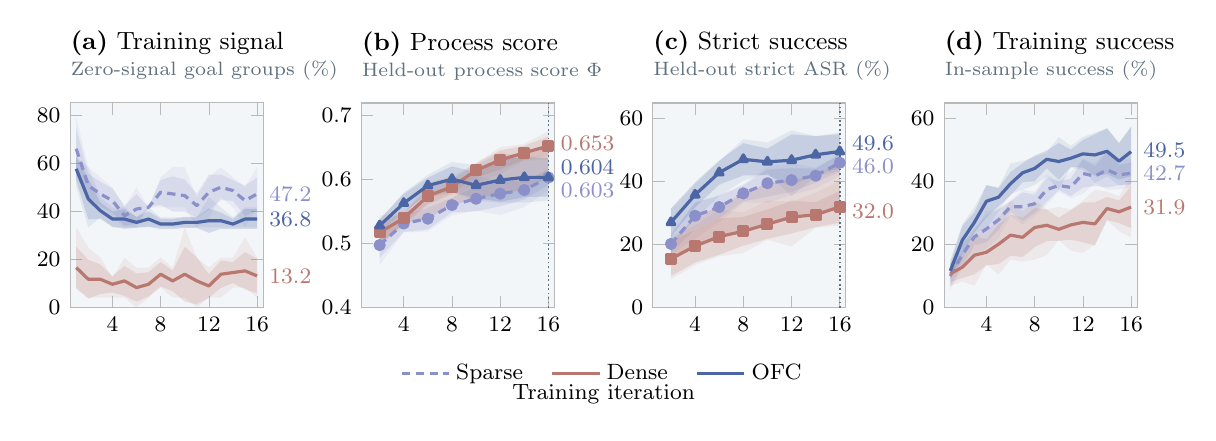
\begin{tikzpicture}\begin{groupplot}[group style={group size=4 by 1,horizontal sep=1.25cm},width=2.45cm,height=2.6cm,xmin=0.5,xmax=16.5,xtick={4,8,12,16},xlabel={},scale only axis,clip mode=individual,axis background/.style={fill=diagramlight},axis line style={gray!55},tick style={gray!55},tick label style={font=\footnotesize},title style={at={(0,1)},anchor=south west,align=left,font=\small,yshift=1pt,inner ysep=1pt,inner xsep=0pt},xlabel style={font=\footnotesize,yshift=2pt},every axis plot/.append style={line join=round},legend style={font=\fontsize{8pt}{9.5pt}\selectfont,draw=none,fill=none,/tikz/every even column/.append style={column sep=0.8em}}]
\nextgroupplot[title={\textbf{(a)} Training signal\\[-1.5pt]{\scriptsize\color{diagrammuted}Zero-signal goal groups (\%)}},ymin=0,ymax=85]
\addplot[name path=sparseamma,draw=none,forget plot] coordinates {(1.00000,54.16670) (2.00000,45.83330) (3.00000,41.66670) (4.00000,37.50000) (5.00000,33.33330) (6.00000,33.33330) (7.00000,41.66670) (8.00000,41.66670) (9.00000,41.66670) (10.00000,41.66670) (11.00000,33.33330) (12.00000,37.50000) (13.00000,45.83330) (14.00000,41.66670) (15.00000,33.33330) (16.00000,41.66670)};
\addplot[name path=sparseammb,draw=none,forget plot] coordinates {(1.00000,79.16670) (2.00000,58.33330) (3.00000,54.16670) (4.00000,50.00000) (5.00000,41.66670) (6.00000,50.00000) (7.00000,41.66670) (8.00000,54.16670) (9.00000,58.33330) (10.00000,58.33330) (11.00000,45.83330) (12.00000,54.16670) (13.00000,58.33330) (14.00000,54.16670) (15.00000,50.00000) (16.00000,58.33330)};
\addplot[fill=sparsecolor,fill opacity=0.1,draw=none,forget plot] fill between[of=sparseamma and sparseammb];
\addplot[name path=sparseasda,draw=none,forget plot] coordinates {(1.00000,57.46706) (2.00000,45.82340) (3.00000,42.17615) (4.00000,39.39838) (5.00000,34.09778) (6.00000,34.83905) (7.00000,41.66670) (8.00000,42.81355) (9.00000,39.92563) (10.00000,39.85247) (11.00000,37.49008) (12.00000,40.58050) (13.00000,44.72951) (14.00000,44.30780) (15.00000,38.17132) (16.00000,40.41812)};
\addplot[name path=sparseasdb,draw=none,forget plot] coordinates {(1.00000,74.47740) (2.00000,55.56546) (3.00000,52.26831) (4.00000,49.49052) (5.00000,42.29112) (6.00000,47.10539) (7.00000,41.66670) (8.00000,53.01979) (9.00000,54.51884) (10.00000,53.20310) (11.00000,47.23212) (12.00000,55.25287) (13.00000,55.27046) (14.00000,52.91443) (15.00000,50.71754) (16.00000,54.02634)};
\addplot[fill=sparsecolor,fill opacity=0.18,draw=none,forget plot] fill between[of=sparseasda and sparseasdb];
\addplot[name path=denseamma,draw=none,forget plot] coordinates {(1.00000,8.33330) (2.00000,4.16670) (3.00000,4.16670) (4.00000,4.16670) (5.00000,4.16670) (6.00000,0.00000) (7.00000,4.16670) (8.00000,8.33330) (9.00000,4.16670) (10.00000,4.16670) (11.00000,0.00000) (12.00000,4.16670) (13.00000,4.16670) (14.00000,8.33330) (15.00000,8.33330) (16.00000,4.16670)};
\addplot[name path=denseammb,draw=none,forget plot] coordinates {(1.00000,33.33330) (2.00000,25.00000) (3.00000,20.83330) (4.00000,12.50000) (5.00000,20.83330) (6.00000,16.66670) (7.00000,16.66670) (8.00000,20.83330) (9.00000,16.66670) (10.00000,33.33330) (11.00000,20.83330) (12.00000,16.66670) (13.00000,20.83330) (14.00000,20.83330) (15.00000,29.16670) (16.00000,20.83330)};
\addplot[fill=densecolor,fill opacity=0.1,draw=none,forget plot] fill between[of=denseamma and denseammb];
\addplot[name path=denseasda,draw=none,forget plot] coordinates {(1.00000,7.92660) (2.00000,3.71895) (3.00000,5.67239) (4.00000,6.32015) (5.00000,4.83800) (6.00000,2.44077) (7.00000,4.67615) (8.00000,8.84279) (9.00000,6.80780) (10.00000,2.50341) (11.00000,1.36906) (12.00000,4.15676) (13.00000,8.19616) (14.00000,10.21329) (15.00000,7.51985) (16.00000,6.01777)};
\addplot[name path=denseasdb,draw=none,forget plot] coordinates {(1.00000,25.40673) (2.00000,19.89219) (3.00000,17.93871) (4.00000,13.12428) (5.00000,17.38420) (6.00000,14.22589) (7.00000,14.76831) (8.00000,18.93498) (9.00000,15.41443) (10.00000,25.27436) (11.00000,20.85314) (12.00000,13.89880) (13.00000,19.58164) (14.00000,18.95338) (15.00000,23.03572) (16.00000,20.37110)};
\addplot[fill=densecolor,fill opacity=0.18,draw=none,forget plot] fill between[of=denseasda and denseasdb];
\addplot[name path=sftamma,draw=none,forget plot] coordinates {(1.00000,50.00000) (2.00000,33.33330) (3.00000,37.50000) (4.00000,33.33330) (5.00000,33.33330) (6.00000,33.33330) (7.00000,33.33330) (8.00000,33.33330) (9.00000,33.33330) (10.00000,33.33330) (11.00000,33.33330) (12.00000,33.33330) (13.00000,33.33330) (14.00000,33.33330) (15.00000,33.33330) (16.00000,33.33330)};
\addplot[name path=sftammb,draw=none,forget plot] coordinates {(1.00000,62.50000) (2.00000,58.33330) (3.00000,45.83330) (4.00000,41.66670) (5.00000,41.66670) (6.00000,37.50000) (7.00000,41.66670) (8.00000,37.50000) (9.00000,37.50000) (10.00000,37.50000) (11.00000,37.50000) (12.00000,45.83330) (13.00000,41.66670) (14.00000,37.50000) (15.00000,41.66670) (16.00000,41.66670)};
\addplot[fill=ofccolor,fill opacity=0.1,draw=none,forget plot] fill between[of=sftamma and sftammb];
\addplot[name path=sftasda,draw=none,forget plot] coordinates {(1.00000,52.76787) (2.00000,36.63372) (3.00000,36.87572) (4.00000,33.66897) (5.00000,32.70888) (6.00000,33.13445) (7.00000,33.66897) (8.00000,32.57053) (9.00000,32.57053) (10.00000,33.13445) (11.00000,33.13445) (12.00000,31.06500) (13.00000,32.70900) (14.00000,32.57053) (15.00000,32.70888) (16.00000,32.70888)};
\addplot[name path=sftasdb,draw=none,forget plot] coordinates {(1.00000,62.50990) (2.00000,53.64405) (3.00000,43.67985) (4.00000,39.94213) (5.00000,40.90222) (6.00000,37.69885) (7.00000,39.94213) (8.00000,36.87387) (9.00000,36.87387) (10.00000,37.69885) (11.00000,37.69885) (12.00000,41.15717) (13.00000,39.51320) (14.00000,36.87387) (15.00000,40.90222) (16.00000,40.90222)};
\addplot[fill=ofccolor,fill opacity=0.18,draw=none,forget plot] fill between[of=sftasda and sftasdb];
\addplot[sparsecolor,line width=1.15pt,mark=none,mark size=1.6pt,mark options={solid},densely dashed] coordinates {(1.00000,65.97223) (2.00000,50.69443) (3.00000,47.22223) (4.00000,44.44445) (5.00000,38.19445) (6.00000,40.97222) (7.00000,41.66670) (8.00000,47.91667) (9.00000,47.22223) (10.00000,46.52778) (11.00000,42.36110) (12.00000,47.91668) (13.00000,49.99998) (14.00000,48.61112) (15.00000,44.44443) (16.00000,47.22223)};
\addplot[densecolor,line width=1.15pt,mark=none,mark size=1.6pt,mark options={solid}] coordinates {(1.00000,16.66667) (2.00000,11.80557) (3.00000,11.80555) (4.00000,9.72222) (5.00000,11.11110) (6.00000,8.33333) (7.00000,9.72223) (8.00000,13.88888) (9.00000,11.11112) (10.00000,13.88888) (11.00000,11.11110) (12.00000,9.02778) (13.00000,13.88890) (14.00000,14.58333) (15.00000,15.27778) (16.00000,13.19443)};
\addplot[ofccolor,line width=1.15pt,mark=none,mark size=1.6pt,mark options={solid}] coordinates {(1.00000,57.63888) (2.00000,45.13888) (3.00000,40.27778) (4.00000,36.80555) (5.00000,36.80555) (6.00000,35.41665) (7.00000,36.80555) (8.00000,34.72220) (9.00000,34.72220) (10.00000,35.41665) (11.00000,35.41665) (12.00000,36.11108) (13.00000,36.11110) (14.00000,34.72220) (15.00000,36.80555) (16.00000,36.80555)};
\node[font=\footnotesize,text=sparsecolor,anchor=west,inner sep=1pt] at (axis cs:16.75,47.22223) {47.2};
\node[font=\footnotesize,text=densecolor,anchor=west,inner sep=1pt] at (axis cs:16.75,13.19443) {13.2};
\node[font=\footnotesize,text=ofccolor,anchor=west,inner sep=1pt] at (axis cs:16.75,36.80555) {36.8};
\nextgroupplot[title={\textbf{(b)} Process score\\[-1.5pt]{\scriptsize\color{diagrammuted}Held-out process score $\Phi$}},ymin=0.4,ymax=0.72]
\draw[densely dotted,diagrammuted,line width=.6pt] (axis cs:16,0.4) -- (axis cs:16,0.72);
\addplot[name path=sparsebmma,draw=none,forget plot] coordinates {(2.00000,0.46700) (4.00000,0.51750) (6.00000,0.51910) (8.00000,0.54430) (10.00000,0.55160) (12.00000,0.54480) (14.00000,0.55710) (16.00000,0.58440)};
\addplot[name path=sparsebmmb,draw=none,forget plot] coordinates {(2.00000,0.52520) (4.00000,0.54880) (6.00000,0.56600) (8.00000,0.57170) (10.00000,0.60470) (12.00000,0.59970) (14.00000,0.59690) (16.00000,0.61680)};
\addplot[fill=sparsecolor,fill opacity=0.1,draw=none,forget plot] fill between[of=sparsebmma and sparsebmmb];
\addplot[name path=sparsebsda,draw=none,forget plot] coordinates {(2.00000,0.47779) (4.00000,0.51841) (6.00000,0.52236) (8.00000,0.54911) (10.00000,0.55051) (12.00000,0.55832) (14.00000,0.56908) (16.00000,0.59225)};
\addplot[name path=sparsebsdb,draw=none,forget plot] coordinates {(2.00000,0.51784) (4.00000,0.54463) (6.00000,0.55584) (8.00000,0.57175) (10.00000,0.58986) (12.00000,0.59818) (14.00000,0.59862) (16.00000,0.61465)};
\addplot[fill=sparsecolor,fill opacity=0.18,draw=none,forget plot] fill between[of=sparsebsda and sparsebsdb];
\addplot[name path=densebmma,draw=none,forget plot] coordinates {(2.00000,0.49640) (4.00000,0.52690) (6.00000,0.56230) (8.00000,0.57480) (10.00000,0.59460) (12.00000,0.60870) (14.00000,0.62970) (16.00000,0.63140)};
\addplot[name path=densebmmb,draw=none,forget plot] coordinates {(2.00000,0.54460) (4.00000,0.54790) (6.00000,0.59620) (8.00000,0.60500) (10.00000,0.62590) (12.00000,0.65070) (14.00000,0.65610) (16.00000,0.67600)};
\addplot[fill=densecolor,fill opacity=0.1,draw=none,forget plot] fill between[of=densebmma and densebmmb];
\addplot[name path=densebsda,draw=none,forget plot] coordinates {(2.00000,0.49922) (4.00000,0.53192) (6.00000,0.56214) (8.00000,0.57824) (10.00000,0.60350) (12.00000,0.61607) (14.00000,0.63120) (16.00000,0.63748)};
\addplot[name path=densebsdb,draw=none,forget plot] coordinates {(2.00000,0.53601) (4.00000,0.54812) (6.00000,0.58646) (8.00000,0.60029) (10.00000,0.62567) (12.00000,0.64577) (14.00000,0.65310) (16.00000,0.66789)};
\addplot[fill=densecolor,fill opacity=0.18,draw=none,forget plot] fill between[of=densebsda and densebsdb];
\addplot[name path=sftbmma,draw=none,forget plot] coordinates {(2.00000,0.51460) (4.00000,0.53700) (6.00000,0.57150) (8.00000,0.57990) (10.00000,0.56720) (12.00000,0.56420) (14.00000,0.56440) (16.00000,0.56720)};
\addplot[name path=sftbmmb,draw=none,forget plot] coordinates {(2.00000,0.53770) (4.00000,0.57990) (6.00000,0.60750) (8.00000,0.62780) (10.00000,0.62260) (12.00000,0.64200) (14.00000,0.63660) (16.00000,0.63580)};
\addplot[fill=ofccolor,fill opacity=0.1,draw=none,forget plot] fill between[of=sftbmma and sftbmmb];
\addplot[name path=sftbsda,draw=none,forget plot] coordinates {(2.00000,0.51862) (4.00000,0.54874) (6.00000,0.57855) (8.00000,0.58080) (10.00000,0.57105) (12.00000,0.56563) (14.00000,0.57289) (16.00000,0.57374)};
\addplot[name path=sftbsdb,draw=none,forget plot] coordinates {(2.00000,0.53788) (4.00000,0.57789) (6.00000,0.60315) (8.00000,0.62097) (10.00000,0.61152) (12.00000,0.63333) (14.00000,0.63441) (16.00000,0.63346)};
\addplot[fill=ofccolor,fill opacity=0.18,draw=none,forget plot] fill between[of=sftbsda and sftbsdb];
\addplot[name path=gapba,draw=none,forget plot] coordinates {(2.00000,0.49782) (4.00000,0.53152) (6.00000,0.53910) (8.00000,0.56043) (10.00000,0.57018) (12.00000,0.57825) (14.00000,0.58385) (16.00000,0.60345)};
\addplot[name path=gapbb,draw=none,forget plot] coordinates {(2.00000,0.51762) (4.00000,0.54002) (6.00000,0.57430) (8.00000,0.58927) (10.00000,0.61458) (12.00000,0.63092) (14.00000,0.64215) (16.00000,0.65268)};
\addplot[fill=densecolor,fill opacity=0.22,draw=none,forget plot] fill between[of=gapba and gapbb];
\addplot[sparsecolor,line width=1.15pt,mark=*,mark size=1.6pt,mark options={solid},densely dashed] coordinates {(2.00000,0.49782) (4.00000,0.53152) (6.00000,0.53910) (8.00000,0.56043) (10.00000,0.57018) (12.00000,0.57825) (14.00000,0.58385) (16.00000,0.60345)};
\addplot[densecolor,line width=1.15pt,mark=square*,mark size=1.6pt,mark options={solid}] coordinates {(2.00000,0.51762) (4.00000,0.54002) (6.00000,0.57430) (8.00000,0.58927) (10.00000,0.61458) (12.00000,0.63092) (14.00000,0.64215) (16.00000,0.65268)};
\addplot[ofccolor,line width=1.15pt,mark=triangle*,mark size=1.6pt,mark options={solid}] coordinates {(2.00000,0.52825) (4.00000,0.56332) (6.00000,0.59085) (8.00000,0.60088) (10.00000,0.59128) (12.00000,0.59948) (14.00000,0.60365) (16.00000,0.60360)};
\node[font=\footnotesize,text=sparsecolor,anchor=west,inner sep=1pt] at (axis cs:16.75,0.58314) {0.603};
\node[font=\footnotesize,text=densecolor,anchor=west,inner sep=1pt] at (axis cs:16.75,0.65668) {0.653};
\node[font=\footnotesize,text=ofccolor,anchor=west,inner sep=1pt] at (axis cs:16.75,0.61991) {0.604};
\nextgroupplot[title={\textbf{(c)} Strict success\\[-1.5pt]{\scriptsize\color{diagrammuted}Held-out strict ASR (\%)}},ymin=0,ymax=65]
\draw[densely dotted,diagrammuted,line width=.6pt] (axis cs:16,0) -- (axis cs:16,65);
\addplot[name path=sparsecmma,draw=none,forget plot] coordinates {(2.00000,17.01000) (4.00000,21.88000) (6.00000,27.08000) (8.00000,33.33000) (10.00000,33.33000) (12.00000,35.76000) (14.00000,37.85000) (16.00000,42.01000)};
\addplot[name path=sparsecmmb,draw=none,forget plot] coordinates {(2.00000,23.61000) (4.00000,33.33000) (6.00000,35.76000) (8.00000,39.24000) (10.00000,44.79000) (12.00000,45.83000) (14.00000,44.44000) (16.00000,48.61000)};
\addplot[fill=sparsecolor,fill opacity=0.1,draw=none,forget plot] fill between[of=sparsecmma and sparsecmmb];
\addplot[name path=sparsecsda,draw=none,forget plot] coordinates {(2.00000,17.49607) (4.00000,24.93858) (6.00000,28.40187) (8.00000,33.78339) (10.00000,35.23501) (12.00000,36.74356) (14.00000,39.67508) (16.00000,43.25735)};
\addplot[name path=sparsecsdb,draw=none,forget plot] coordinates {(2.00000,23.01060) (4.00000,33.39142) (6.00000,35.48480) (8.00000,38.78994) (10.00000,43.81499) (12.00000,44.27310) (14.00000,44.12159) (16.00000,48.75598)};
\addplot[fill=sparsecolor,fill opacity=0.18,draw=none,forget plot] fill between[of=sparsecsda and sparsecsdb];
\addplot[name path=densecmma,draw=none,forget plot] coordinates {(2.00000,9.03000) (4.00000,13.54000) (6.00000,16.32000) (8.00000,17.36000) (10.00000,21.53000) (12.00000,19.44000) (14.00000,25.35000) (16.00000,26.04000)};
\addplot[name path=densecmmb,draw=none,forget plot] coordinates {(2.00000,22.57000) (4.00000,26.04000) (6.00000,31.25000) (8.00000,30.21000) (10.00000,34.03000) (12.00000,33.68000) (14.00000,36.46000) (16.00000,40.28000)};
\addplot[fill=densecolor,fill opacity=0.1,draw=none,forget plot] fill between[of=densecmma and densecmmb];
\addplot[name path=densecsda,draw=none,forget plot] coordinates {(2.00000,10.05845) (4.00000,14.36791) (6.00000,16.78826) (8.00000,19.68983) (10.00000,21.82925) (12.00000,23.54585) (14.00000,25.57421) (16.00000,26.95731)};
\addplot[name path=densecsdb,draw=none,forget plot] coordinates {(2.00000,20.96155) (4.00000,24.74876) (6.00000,28.35174) (8.00000,28.80351) (10.00000,31.18409) (12.00000,33.97415) (14.00000,33.45579) (16.00000,37.04602)};
\addplot[fill=densecolor,fill opacity=0.18,draw=none,forget plot] fill between[of=densecsda and densecsdb];
\addplot[name path=sftcmma,draw=none,forget plot] coordinates {(2.00000,19.44000) (4.00000,28.12000) (6.00000,35.42000) (8.00000,40.28000) (10.00000,42.71000) (12.00000,35.42000) (14.00000,41.67000) (16.00000,43.40000)};
\addplot[name path=sftcmmb,draw=none,forget plot] coordinates {(2.00000,31.25000) (4.00000,39.24000) (6.00000,46.53000) (8.00000,53.47000) (10.00000,52.43000) (12.00000,56.25000) (14.00000,54.51000) (16.00000,55.56000)};
\addplot[fill=ofccolor,fill opacity=0.1,draw=none,forget plot] fill between[of=sftcmma and sftcmmb];
\addplot[name path=sftcsda,draw=none,forget plot] coordinates {(2.00000,22.65190) (4.00000,31.83950) (6.00000,39.06291) (8.00000,41.98369) (10.00000,42.10603) (12.00000,38.62185) (14.00000,42.66330) (16.00000,44.10889)};
\addplot[name path=sftcsdb,draw=none,forget plot] coordinates {(2.00000,31.51477) (4.00000,39.80383) (6.00000,46.70376) (8.00000,52.22964) (10.00000,50.49064) (12.00000,55.01482) (14.00000,54.44003) (16.00000,55.07777)};
\addplot[fill=ofccolor,fill opacity=0.18,draw=none,forget plot] fill between[of=sftcsda and sftcsdb];
\addplot[name path=gapca,draw=none,forget plot] coordinates {(2.00000,20.25333) (4.00000,29.16500) (6.00000,31.94333) (8.00000,36.28667) (10.00000,39.52500) (12.00000,40.50833) (14.00000,41.89833) (16.00000,46.00667)};
\addplot[name path=gapcb,draw=none,forget plot] coordinates {(2.00000,15.51000) (4.00000,19.55833) (6.00000,22.57000) (8.00000,24.24667) (10.00000,26.50667) (12.00000,28.76000) (14.00000,29.51500) (16.00000,32.00167)};
\addplot[fill=densecolor,fill opacity=0.22,draw=none,forget plot] fill between[of=gapca and gapcb];
\addplot[sparsecolor,line width=1.15pt,mark=*,mark size=1.6pt,mark options={solid},densely dashed] coordinates {(2.00000,20.25333) (4.00000,29.16500) (6.00000,31.94333) (8.00000,36.28667) (10.00000,39.52500) (12.00000,40.50833) (14.00000,41.89833) (16.00000,46.00667)};
\addplot[densecolor,line width=1.15pt,mark=square*,mark size=1.6pt,mark options={solid}] coordinates {(2.00000,15.51000) (4.00000,19.55833) (6.00000,22.57000) (8.00000,24.24667) (10.00000,26.50667) (12.00000,28.76000) (14.00000,29.51500) (16.00000,32.00167)};
\addplot[ofccolor,line width=1.15pt,mark=triangle*,mark size=1.6pt,mark options={solid}] coordinates {(2.00000,27.08333) (4.00000,35.82167) (6.00000,42.88333) (8.00000,47.10667) (10.00000,46.29833) (12.00000,46.81833) (14.00000,48.55167) (16.00000,49.59333)};
\node[font=\footnotesize,text=sparsecolor,anchor=west,inner sep=1pt] at (axis cs:16.75,44.71272) {46.0};
\node[font=\footnotesize,text=densecolor,anchor=west,inner sep=1pt] at (axis cs:16.75,30.70772) {32.0};
\node[font=\footnotesize,text=ofccolor,anchor=west,inner sep=1pt] at (axis cs:16.75,52.18123) {49.6};
\nextgroupplot[title={\textbf{(d)} Training success\\[-1.5pt]{\scriptsize\color{diagrammuted}In-sample success (\%)}},ymin=0,ymax=65,legend to name=coreleg,legend columns=3]
\addplot[name path=sparsedmma,draw=none,forget plot] coordinates {(1.00000,5.55560) (2.00000,12.50000) (3.00000,17.36110) (4.00000,18.75000) (5.00000,22.22220) (6.00000,29.16670) (7.00000,26.38890) (8.00000,29.16670) (9.00000,32.63890) (10.00000,36.80560) (11.00000,34.72220) (12.00000,36.11110) (13.00000,39.58330) (14.00000,37.50000) (15.00000,37.50000) (16.00000,38.19440)};
\addplot[name path=sparsedmmb,draw=none,forget plot] coordinates {(1.00000,14.58330) (2.00000,20.13890) (3.00000,24.30560) (4.00000,30.55560) (5.00000,31.25000) (6.00000,34.02780) (7.00000,37.50000) (8.00000,36.80560) (9.00000,42.36110) (10.00000,40.27780) (11.00000,43.05560) (12.00000,47.22220) (13.00000,45.83330) (14.00000,50.69440) (15.00000,47.22220) (16.00000,47.22220)};
\addplot[fill=sparsecolor,fill opacity=0.1,draw=none,forget plot] fill between[of=sparsedmma and sparsedmmb];
\addplot[name path=sparsedsda,draw=none,forget plot] coordinates {(1.00000,6.59029) (2.00000,13.39689) (3.00000,19.83070) (4.00000,20.78729) (5.00000,24.59460) (6.00000,30.45143) (7.00000,27.50817) (8.00000,30.04803) (9.00000,33.69639) (10.00000,37.42537) (11.00000,35.41665) (12.00000,38.14237) (13.00000,38.63305) (14.00000,38.17709) (15.00000,38.91213) (16.00000,39.34185)};
\addplot[name path=sparsedsdb,draw=none,forget plot] coordinates {(1.00000,13.54857) (2.00000,20.16787) (3.00000,25.07674) (4.00000,29.21271) (5.00000,31.19247) (6.00000,33.66893) (7.00000,36.61220) (8.00000,35.92420) (9.00000,41.30361) (10.00000,40.12093) (11.00000,40.97225) (12.00000,47.04280) (13.00000,44.93172) (14.00000,49.32288) (15.00000,45.34714) (16.00000,46.07475)};
\addplot[fill=sparsecolor,fill opacity=0.18,draw=none,forget plot] fill between[of=sparsedsda and sparsedsdb];
\addplot[name path=densedmma,draw=none,forget plot] coordinates {(1.00000,6.94440) (2.00000,8.33330) (3.00000,6.94440) (4.00000,13.88890) (5.00000,10.41670) (6.00000,15.27780) (7.00000,14.58330) (8.00000,15.27780) (9.00000,16.66670) (10.00000,21.52780) (11.00000,18.05560) (12.00000,17.36110) (13.00000,20.13890) (14.00000,27.77780) (15.00000,24.30560) (16.00000,22.22220)};
\addplot[name path=densedmmb,draw=none,forget plot] coordinates {(1.00000,13.88890) (2.00000,17.36110) (3.00000,23.61110) (4.00000,24.30560) (5.00000,28.47220) (6.00000,34.02780) (7.00000,30.55560) (8.00000,34.02780) (9.00000,31.25000) (10.00000,31.94440) (11.00000,31.25000) (12.00000,34.02780) (13.00000,37.50000) (14.00000,36.80560) (15.00000,35.41670) (16.00000,41.66670)};
\addplot[fill=densecolor,fill opacity=0.1,draw=none,forget plot] fill between[of=densedmma and densedmmb];
\addplot[name path=densedsda,draw=none,forget plot] coordinates {(1.00000,8.10133) (2.00000,9.45225) (3.00000,10.56502) (4.00000,13.43365) (5.00000,13.85044) (6.00000,16.49703) (7.00000,16.10470) (8.00000,19.22584) (9.00000,21.15613) (10.00000,21.22498) (11.00000,21.59575) (12.00000,20.76426) (13.00000,19.76447) (14.00000,27.78938) (15.00000,26.86047) (16.00000,25.26907)};
\addplot[name path=densedsdb,draw=none,forget plot] coordinates {(1.00000,13.42643) (2.00000,16.24218) (3.00000,22.76828) (4.00000,21.75155) (5.00000,26.42733) (6.00000,29.56784) (7.00000,28.57123) (8.00000,31.70010) (9.00000,31.15867) (10.00000,28.54355) (11.00000,30.95055) (12.00000,33.40241) (13.00000,33.47630) (14.00000,35.17362) (15.00000,34.01919) (16.00000,38.61979)};
\addplot[fill=densecolor,fill opacity=0.18,draw=none,forget plot] fill between[of=densedsda and densedsdb];
\addplot[name path=sftdmma,draw=none,forget plot] coordinates {(1.00000,9.02780) (2.00000,15.27780) (3.00000,23.61110) (4.00000,25.00000) (5.00000,30.55560) (6.00000,36.11110) (7.00000,37.50000) (8.00000,38.88890) (9.00000,41.66670) (10.00000,37.50000) (11.00000,44.44440) (12.00000,43.75000) (13.00000,39.58330) (14.00000,41.66670) (15.00000,38.88890) (16.00000,38.88890)};
\addplot[name path=sftdmmb,draw=none,forget plot] coordinates {(1.00000,15.27780) (2.00000,26.38890) (3.00000,31.94440) (4.00000,38.88890) (5.00000,38.19440) (6.00000,45.83330) (7.00000,46.52780) (8.00000,47.91670) (9.00000,49.30560) (10.00000,54.16670) (11.00000,51.38890) (12.00000,54.16670) (13.00000,55.55560) (14.00000,56.94440) (15.00000,52.08330) (16.00000,57.63890)};
\addplot[fill=ofccolor,fill opacity=0.1,draw=none,forget plot] fill between[of=sftdmma and sftdmmb];
\addplot[name path=sftdsda,draw=none,forget plot] coordinates {(1.00000,9.47558) (2.00000,16.83890) (3.00000,23.91617) (4.00000,28.68063) (5.00000,32.19779) (6.00000,35.63370) (7.00000,39.82374) (8.00000,40.14783) (9.00000,44.27997) (10.00000,40.54544) (11.00000,44.72258) (12.00000,44.45787) (13.00000,41.91582) (14.00000,42.35947) (15.00000,40.70107) (16.00000,41.68438)};
\addplot[name path=sftdsdb,draw=none,forget plot] coordinates {(1.00000,13.90409) (2.00000,25.98516) (3.00000,30.25046) (4.00000,38.91201) (5.00000,37.94111) (6.00000,43.06997) (7.00000,45.82443) (8.00000,48.27811) (9.00000,49.93303) (10.00000,52.27863) (11.00000,50.18482) (12.00000,53.22733) (13.00000,55.07491) (14.00000,56.94609) (15.00000,52.35446) (16.00000,57.38972)};
\addplot[fill=ofccolor,fill opacity=0.18,draw=none,forget plot] fill between[of=sftdsda and sftdsdb];
\addplot[sparsecolor,line width=1.15pt,mark=none,mark size=1.6pt,mark options={solid},densely dashed] coordinates {(1.00000,10.06943) (2.00000,16.78238) (3.00000,22.45372) (4.00000,25.00000) (5.00000,27.89353) (6.00000,32.06018) (7.00000,32.06018) (8.00000,32.98612) (9.00000,37.50000) (10.00000,38.77315) (11.00000,38.19445) (12.00000,42.59258) (13.00000,41.78238) (14.00000,43.74998) (15.00000,42.12963) (16.00000,42.70830)};
\addlegendentry{Sparse}
\addplot[densecolor,line width=1.15pt,mark=none,mark size=1.6pt,mark options={solid}] coordinates {(1.00000,10.76388) (2.00000,12.84722) (3.00000,16.66665) (4.00000,17.59260) (5.00000,20.13888) (6.00000,23.03243) (7.00000,22.33797) (8.00000,25.46297) (9.00000,26.15740) (10.00000,24.88427) (11.00000,26.27315) (12.00000,27.08333) (13.00000,26.62038) (14.00000,31.48150) (15.00000,30.43983) (16.00000,31.94443)};
\addlegendentry{Dense}
\addplot[ofccolor,line width=1.15pt,mark=none,mark size=1.6pt,mark options={solid}] coordinates {(1.00000,11.68983) (2.00000,21.41203) (3.00000,27.08332) (4.00000,33.79632) (5.00000,35.06945) (6.00000,39.35183) (7.00000,42.82408) (8.00000,44.21297) (9.00000,47.10650) (10.00000,46.41203) (11.00000,47.45370) (12.00000,48.84260) (13.00000,48.49537) (14.00000,49.65278) (15.00000,46.52777) (16.00000,49.53705)};
\addlegendentry{OFC}
\node[font=\footnotesize,text=sparsecolor,anchor=west,inner sep=1pt] at (axis cs:16.75,42.49505) {42.7};
\node[font=\footnotesize,text=densecolor,anchor=west,inner sep=1pt] at (axis cs:16.75,31.73118) {31.9};
\node[font=\footnotesize,text=ofccolor,anchor=west,inner sep=1pt] at (axis cs:16.75,49.96356) {49.5};
\end{groupplot}
\node[anchor=north] at ($(group c1r1.south west)!0.5!(group c4r1.south east)+(0,-0.45cm)$) {\pgfplotslegendfromname{coreleg}};
\node[anchor=north,font=\footnotesize] at ($(group c1r1.south west)!0.5!(group c4r1.south east)+(0,-0.85cm)$) {Training iteration};
\end{tikzpicture}
}
\section*{Figure 5: budget dependence}
\noindent\resizebox{\linewidth}{!}{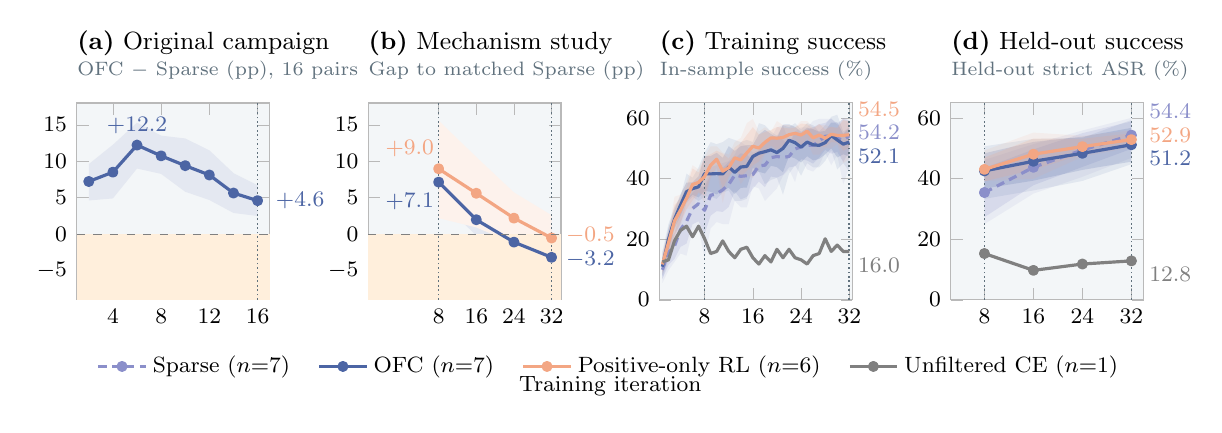
\begin{tikzpicture}\begin{groupplot}[group style={group size=4 by 1,horizontal sep=1.25cm},width=2.45cm,height=2.5cm,xlabel={},scale only axis,clip mode=individual,axis background/.style={fill=diagramlight},axis line style={gray!55},tick style={gray!55},tick label style={font=\footnotesize},title style={at={(0,1)},anchor=south west,align=left,font=\small,yshift=1pt,inner ysep=1pt,inner xsep=0pt},xlabel style={font=\footnotesize,yshift=2pt},every axis plot/.append style={line join=round},legend style={font=\fontsize{8pt}{9.5pt}\selectfont,draw=none,fill=none,/tikz/every even column/.append style={column sep=0.8em}}]
\nextgroupplot[title={\textbf{(a)} Original campaign\\[-1.5pt]{\scriptsize\color{diagrammuted}OFC $-$ Sparse (pp), 16 pairs}},ymin=-9,ymax=18,ytick={-5,0,5,10,15},xmin=1,xmax=17,xtick={4,8,12,16}]
\fill[highlightcolor!40] (axis cs:1,-9) rectangle (axis cs:17,0);
\draw[densely dotted,diagrammuted,line width=.6pt] (axis cs:16,-9) -- (axis cs:16,18);
\addplot[name path=origlo,draw=none,forget plot] coordinates {(2.00000,4.62400) (4.00000,4.90400) (6.00000,9.00400) (8.00000,8.26600) (10.00000,5.81700) (12.00000,4.68700) (14.00000,2.90800) (16.00000,2.49500)};
\addplot[name path=orighi,draw=none,forget plot] coordinates {(2.00000,9.61400) (4.00000,12.26500) (6.00000,15.30000) (8.00000,13.51700) (10.00000,13.13000) (12.00000,11.50400) (14.00000,8.37600) (16.00000,6.70700)};
\addplot[ofccolor!15,forget plot] fill between[of=origlo and orighi];
\addplot[ofccolor,line width=1.15pt,mark=*,mark size=1.4pt,forget plot] coordinates {(2.00000,7.22750) (4.00000,8.50810) (6.00000,12.21940) (8.00000,10.74060) (10.00000,9.39750) (12.00000,8.11810) (14.00000,5.64190) (16.00000,4.60120)};
\addplot[gray,dashed,forget plot] coordinates {(1,0)(17,0)};
\node[font=\footnotesize,text=ofccolor,anchor=south,inner sep=1pt,yshift=3pt] at (axis cs:6.00,12.21940) {$+$12.2};
\node[font=\footnotesize,text=ofccolor,anchor=west,inner sep=1pt] at (axis cs:17.25,4.60120) {$+$4.6};
\nextgroupplot[title={\textbf{(b)} Mechanism study\\[-1.5pt]{\scriptsize\color{diagrammuted}Gap to matched Sparse (pp)}},ymin=-9,ymax=18,ytick={-5,0,5,10,15},xmin=-7,xmax=34,xtick={8,16,24,32}]
\fill[highlightcolor!40] (axis cs:-7,-9) rectangle (axis cs:34,0);
\draw[densely dotted,diagrammuted,line width=.6pt] (axis cs:8,-9) -- (axis cs:8,18);
\draw[densely dotted,diagrammuted,line width=.6pt] (axis cs:32,-9) -- (axis cs:32,18);
\addplot[name path=sftlo,draw=none,forget plot] coordinates {(8.00000,4.86000) (16.00000,-0.20100) (24.00000,-4.80900) (32.00000,-7.09400)};
\addplot[name path=sfthi,draw=none,forget plot] coordinates {(8.00000,9.32400) (16.00000,4.36600) (24.00000,2.63100) (32.00000,1.24000)};
\addplot[ofccolor!15,forget plot] fill between[of=sftlo and sfthi];
\addplot[ofccolor,line width=1.15pt,mark=*,mark size=1.4pt,forget plot] coordinates {(8.00000,7.14290) (16.00000,1.98290) (24.00000,-1.08860) (32.00000,-3.17570)};
\node[font=\footnotesize,text=ofccolor,anchor=north east,inner sep=1pt,yshift=-3pt] at (axis cs:7.70,7.14290) {$+$7.1};
\addplot[name path=rl_poslo,draw=none,forget plot] coordinates {(8.00000,2.20000) (16.00000,0.92500) (24.00000,-1.27300) (32.00000,-3.87700)};
\addplot[name path=rl_poshi,draw=none,forget plot] coordinates {(8.00000,15.57200) (16.00000,10.58800) (24.00000,5.73000) (32.00000,2.60000)};
\addplot[poscolor!15,forget plot] fill between[of=rl_poslo and rl_poshi];
\addplot[poscolor,line width=1.15pt,mark=*,mark size=1.4pt,forget plot] coordinates {(8.00000,8.97170) (16.00000,5.61170) (24.00000,2.20000) (32.00000,-0.52330)};
\node[font=\footnotesize,text=poscolor,anchor=south east,inner sep=1pt,yshift=3pt] at (axis cs:7.70,8.97170) {$+$9.0};
\addplot[gray,dashed,forget plot] coordinates {(-7,0)(34,0)};
\node[font=\footnotesize,text=ofccolor,anchor=west,inner sep=1pt] at (axis cs:34.40,-3.46270) {$-$3.2};
\node[font=\footnotesize,text=poscolor,anchor=west,inner sep=1pt] at (axis cs:34.40,-0.23630) {$-$0.5};
\nextgroupplot[title={\textbf{(c)} Training success\\[-1.5pt]{\scriptsize\color{diagrammuted}In-sample success (\%)}},ymin=0,ymax=65,xmin=0.5,xmax=32.5,xtick={8,16,24,32}]
\draw[densely dotted,diagrammuted,line width=.6pt] (axis cs:8,0) -- (axis cs:8,65);
\draw[densely dotted,diagrammuted,line width=.6pt] (axis cs:32,0) -- (axis cs:32,65);
\addplot[name path=sparsetrnmma,draw=none,forget plot] coordinates {(1.00000,5.55560) (2.00000,9.72220) (3.00000,12.50000) (4.00000,15.27780) (5.00000,14.58330) (6.00000,22.91670) (7.00000,23.61110) (8.00000,13.88890) (9.00000,23.61110) (10.00000,25.69440) (11.00000,25.00000) (12.00000,25.00000) (13.00000,32.63890) (14.00000,30.55560) (15.00000,30.55560) (16.00000,37.50000) (17.00000,36.80560) (18.00000,32.63890) (19.00000,34.72220) (20.00000,36.80560) (21.00000,40.97220) (22.00000,43.05560) (23.00000,38.88890) (24.00000,46.52780) (25.00000,43.05560) (26.00000,42.36110) (27.00000,44.44440) (28.00000,48.61110) (29.00000,44.44440) (30.00000,47.91670) (31.00000,38.19440) (32.00000,43.75000)};
\addplot[name path=sparsetrnmmb,draw=none,forget plot] coordinates {(1.00000,15.27780) (2.00000,21.52780) (3.00000,24.30560) (4.00000,31.25000) (5.00000,34.72220) (6.00000,37.50000) (7.00000,36.11110) (8.00000,37.50000) (9.00000,43.75000) (10.00000,44.44440) (11.00000,45.13890) (12.00000,45.83330) (13.00000,47.91670) (14.00000,52.08330) (15.00000,50.69440) (16.00000,48.61110) (17.00000,49.30560) (18.00000,52.77780) (19.00000,53.47220) (20.00000,56.94440) (21.00000,57.63890) (22.00000,52.08330) (23.00000,55.55560) (24.00000,56.94440) (25.00000,56.94440) (26.00000,59.02780) (27.00000,59.72220) (28.00000,59.72220) (29.00000,59.72220) (30.00000,58.33330) (31.00000,59.72220) (32.00000,59.02780)};
\addplot[fill=sparsecolor,fill opacity=0.1,draw=none,forget plot] fill between[of=sparsetrnmma and sparsetrnmmb];
\addplot[name path=sparsetrnsda,draw=none,forget plot] coordinates {(1.00000,6.95494) (2.00000,11.46981) (3.00000,13.49860) (4.00000,17.47575) (5.00000,18.57955) (6.00000,24.94876) (7.00000,25.92601) (8.00000,21.80084) (9.00000,27.79432) (10.00000,29.28127) (11.00000,29.01824) (12.00000,30.67596) (13.00000,35.87106) (14.00000,33.14847) (15.00000,33.98165) (16.00000,36.66153) (17.00000,39.05372) (18.00000,37.20533) (19.00000,40.71513) (20.00000,40.36050) (21.00000,41.25929) (22.00000,43.72577) (23.00000,44.07908) (24.00000,46.43263) (25.00000,46.00622) (26.00000,44.96654) (27.00000,46.97025) (28.00000,49.54494) (29.00000,48.23759) (30.00000,48.83237) (31.00000,45.53865) (32.00000,49.07934)};
\addplot[name path=sparsetrnsdb,draw=none,forget plot] coordinates {(1.00000,12.88634) (2.00000,19.68099) (3.00000,22.01728) (4.00000,28.95282) (5.00000,33.20613) (6.00000,35.36870) (7.00000,37.56604) (8.00000,37.32613) (9.00000,41.25328) (10.00000,40.75838) (11.00000,43.60078) (12.00000,45.51453) (13.00000,46.47023) (14.00000,48.39916) (15.00000,47.96278) (16.00000,46.07655) (17.00000,49.43837) (18.00000,51.68358) (19.00000,53.13404) (20.00000,54.28238) (21.00000,52.78834) (22.00000,50.91709) (23.00000,55.52412) (24.00000,54.55943) (25.00000,56.17632) (26.00000,57.01758) (27.00000,57.99007) (28.00000,58.39154) (29.00000,59.89732) (30.00000,57.71523) (31.00000,60.01689) (32.00000,59.25400)};
\addplot[fill=sparsecolor,fill opacity=0.18,draw=none,forget plot] fill between[of=sparsetrnsda and sparsetrnsdb];
\addplot[sparsecolor,line width=1.15pt,mark=none,mark size=1.1pt,mark options={solid},densely dashed] coordinates {(1.00000,9.92064) (2.00000,15.57540) (3.00000,17.75794) (4.00000,23.21429) (5.00000,25.89284) (6.00000,30.15873) (7.00000,31.74603) (8.00000,29.56349) (9.00000,34.52380) (10.00000,35.01983) (11.00000,36.30951) (12.00000,38.09524) (13.00000,41.17064) (14.00000,40.77381) (15.00000,40.97221) (16.00000,41.36904) (17.00000,44.24604) (18.00000,44.44446) (19.00000,46.92459) (20.00000,47.32144) (21.00000,47.02381) (22.00000,47.32143) (23.00000,49.80160) (24.00000,50.49603) (25.00000,51.09127) (26.00000,50.99206) (27.00000,52.48016) (28.00000,53.96824) (29.00000,54.06746) (30.00000,53.27380) (31.00000,52.77777) (32.00000,54.16667)};
\addplot[name path=sfttrnmma,draw=none,forget plot] coordinates {(1.00000,6.94440) (2.00000,13.19440) (3.00000,21.52780) (4.00000,25.00000) (5.00000,31.94440) (6.00000,34.02780) (7.00000,32.63890) (8.00000,34.02780) (9.00000,34.02780) (10.00000,33.33330) (11.00000,35.41670) (12.00000,36.11110) (13.00000,32.63890) (14.00000,32.63890) (15.00000,33.33330) (16.00000,40.97220) (17.00000,42.36110) (18.00000,38.19440) (19.00000,39.58330) (20.00000,40.27780) (21.00000,34.72220) (22.00000,41.66670) (23.00000,44.44440) (24.00000,40.97220) (25.00000,45.13890) (26.00000,43.75000) (27.00000,43.75000) (28.00000,45.83330) (29.00000,49.30560) (30.00000,43.05560) (31.00000,45.13890) (32.00000,42.36110)};
\addplot[name path=sfttrnmmb,draw=none,forget plot] coordinates {(1.00000,15.97220) (2.00000,25.00000) (3.00000,30.55560) (4.00000,34.02780) (5.00000,41.66670) (6.00000,40.27780) (7.00000,43.75000) (8.00000,48.61110) (9.00000,52.08330) (10.00000,51.38890) (11.00000,52.08330) (12.00000,53.47220) (13.00000,52.77780) (14.00000,52.08330) (15.00000,52.77780) (16.00000,52.08330) (17.00000,58.33330) (18.00000,57.63890) (19.00000,55.55560) (20.00000,54.16670) (21.00000,57.63890) (22.00000,56.94440) (23.00000,58.33330) (24.00000,56.25000) (25.00000,58.33330) (26.00000,57.63890) (27.00000,55.55560) (28.00000,57.63890) (29.00000,60.41670) (30.00000,61.11110) (31.00000,55.55560) (32.00000,56.94440)};
\addplot[fill=ofccolor,fill opacity=0.1,draw=none,forget plot] fill between[of=sfttrnmma and sfttrnmmb];
\addplot[name path=sfttrnsda,draw=none,forget plot] coordinates {(1.00000,7.86676) (2.00000,16.14286) (3.00000,23.48905) (4.00000,27.68640) (5.00000,32.71775) (6.00000,34.64521) (7.00000,33.81286) (8.00000,35.94017) (9.00000,35.65549) (10.00000,34.79201) (11.00000,36.27223) (12.00000,36.94623) (13.00000,34.97181) (14.00000,36.98124) (15.00000,37.03569) (16.00000,43.57254) (17.00000,42.27020) (18.00000,41.71575) (19.00000,44.23479) (20.00000,43.81659) (21.00000,42.14324) (22.00000,47.39855) (23.00000,46.67712) (24.00000,45.37536) (25.00000,47.40765) (26.00000,46.02922) (27.00000,46.51201) (28.00000,48.00359) (29.00000,49.99580) (30.00000,47.00932) (31.00000,48.03442) (32.00000,47.35633)};
\addplot[name path=sfttrnsdb,draw=none,forget plot] coordinates {(1.00000,13.95861) (2.00000,23.73806) (3.00000,29.68555) (4.00000,34.81363) (5.00000,38.71082) (6.00000,38.76753) (7.00000,40.79029) (8.00000,47.39320) (9.00000,47.47948) (10.00000,48.54133) (11.00000,46.86268) (12.00000,50.75217) (13.00000,49.15519) (14.00000,50.71713) (15.00000,51.05951) (16.00000,51.07035) (17.00000,54.55520) (18.00000,56.10171) (19.00000,54.77312) (20.00000,53.40561) (21.00000,57.85674) (22.00000,57.95860) (23.00000,57.09271) (24.00000,55.41827) (25.00000,56.75904) (26.00000,56.35178) (27.00000,55.47213) (28.00000,55.76626) (29.00000,58.53600) (30.00000,58.54625) (31.00000,54.74338) (32.00000,56.81030)};
\addplot[fill=ofccolor,fill opacity=0.18,draw=none,forget plot] fill between[of=sfttrnsda and sfttrnsdb];
\addplot[ofccolor,line width=1.15pt,mark=none,mark size=1.1pt,mark options={solid}] coordinates {(1.00000,10.91269) (2.00000,19.94046) (3.00000,26.58730) (4.00000,31.25001) (5.00000,35.71429) (6.00000,36.70637) (7.00000,37.30157) (8.00000,41.66669) (9.00000,41.56749) (10.00000,41.66667) (11.00000,41.56746) (12.00000,43.84920) (13.00000,42.06350) (14.00000,43.84919) (15.00000,44.04760) (16.00000,47.32144) (17.00000,48.41270) (18.00000,48.90873) (19.00000,49.50396) (20.00000,48.61110) (21.00000,49.99999) (22.00000,52.67857) (23.00000,51.88491) (24.00000,50.39681) (25.00000,52.08334) (26.00000,51.19050) (27.00000,50.99207) (28.00000,51.88493) (29.00000,54.26590) (30.00000,52.77779) (31.00000,51.38890) (32.00000,52.08331)};
\addplot[name path=rl_postrnmma,draw=none,forget plot] coordinates {(1.00000,8.33330) (2.00000,13.88890) (3.00000,18.05560) (4.00000,24.30560) (5.00000,29.86110) (6.00000,29.86110) (7.00000,35.41670) (8.00000,31.94440) (9.00000,40.27780) (10.00000,43.05560) (11.00000,31.94440) (12.00000,40.27780) (13.00000,43.05560) (14.00000,38.19440) (15.00000,40.97220) (16.00000,40.27780) (17.00000,43.05560) (18.00000,47.91670) (19.00000,49.30560) (20.00000,49.30560) (21.00000,50.69440) (22.00000,52.08330) (23.00000,52.08330) (24.00000,50.00000) (25.00000,52.08330) (26.00000,47.91670) (27.00000,47.91670) (28.00000,50.00000) (29.00000,50.00000) (30.00000,51.38890) (31.00000,45.13890) (32.00000,46.52780)};
\addplot[name path=rl_postrnmmb,draw=none,forget plot] coordinates {(1.00000,15.97220) (2.00000,22.22220) (3.00000,34.02780) (4.00000,34.72220) (5.00000,38.88890) (6.00000,44.44440) (7.00000,43.05560) (8.00000,47.22220) (9.00000,50.69440) (10.00000,50.69440) (11.00000,48.61110) (12.00000,47.91670) (13.00000,52.08330) (14.00000,53.47220) (15.00000,58.33330) (16.00000,59.72220) (17.00000,55.55560) (18.00000,56.94440) (19.00000,55.55560) (20.00000,59.02780) (21.00000,57.63890) (22.00000,57.63890) (23.00000,56.94440) (24.00000,59.02780) (25.00000,59.02780) (26.00000,56.94440) (27.00000,57.63890) (28.00000,57.63890) (29.00000,56.94440) (30.00000,56.94440) (31.00000,59.72220) (32.00000,59.02780)};
\addplot[fill=poscolor,fill opacity=0.1,draw=none,forget plot] fill between[of=rl_postrnmma and rl_postrnmmb];
\addplot[name path=rl_postrnsda,draw=none,forget plot] coordinates {(1.00000,9.22804) (2.00000,14.94638) (3.00000,20.79416) (4.00000,25.80916) (5.00000,29.95191) (6.00000,32.81893) (7.00000,35.50362) (8.00000,34.41150) (9.00000,40.79615) (10.00000,43.58551) (11.00000,36.70973) (12.00000,40.67436) (13.00000,43.39584) (14.00000,40.61196) (15.00000,42.59600) (16.00000,44.39067) (17.00000,45.67096) (18.00000,48.55375) (19.00000,50.91127) (20.00000,49.69718) (21.00000,50.28901) (22.00000,52.46555) (23.00000,53.14391) (24.00000,50.60299) (25.00000,53.37157) (26.00000,50.49342) (27.00000,50.68002) (28.00000,50.46248) (29.00000,52.08123) (30.00000,51.90029) (31.00000,49.26670) (32.00000,50.23870)};
\addplot[name path=rl_postrnsdb,draw=none,forget plot] coordinates {(1.00000,14.15159) (2.00000,22.55359) (3.00000,31.28921) (4.00000,33.45010) (5.00000,37.17773) (6.00000,43.33847) (7.00000,42.04271) (8.00000,47.06996) (9.00000,48.09272) (10.00000,49.23855) (11.00000,48.24394) (12.00000,46.59414) (13.00000,50.35416) (14.00000,51.74910) (15.00000,54.39473) (16.00000,56.99820) (17.00000,54.56057) (18.00000,55.38145) (19.00000,56.03323) (20.00000,57.01582) (21.00000,56.88689) (22.00000,56.56221) (23.00000,56.80979) (24.00000,58.19334) (25.00000,57.97103) (26.00000,56.45105) (27.00000,58.11628) (28.00000,56.25048) (29.00000,57.17803) (30.00000,56.66451) (31.00000,59.29814) (32.00000,58.78910)};
\addplot[fill=poscolor,fill opacity=0.18,draw=none,forget plot] fill between[of=rl_postrnsda and rl_postrnsdb];
\addplot[poscolor,line width=1.15pt,mark=none,mark size=1.1pt,mark options={solid}] coordinates {(1.00000,11.68982) (2.00000,18.74998) (3.00000,26.04168) (4.00000,29.62963) (5.00000,33.56482) (6.00000,38.07870) (7.00000,38.77317) (8.00000,40.74073) (9.00000,44.44443) (10.00000,46.41203) (11.00000,42.47683) (12.00000,43.63425) (13.00000,46.87500) (14.00000,46.18053) (15.00000,48.49537) (16.00000,50.69443) (17.00000,50.11577) (18.00000,51.96760) (19.00000,53.47225) (20.00000,53.35650) (21.00000,53.58795) (22.00000,54.51388) (23.00000,54.97685) (24.00000,54.39817) (25.00000,55.67130) (26.00000,53.47223) (27.00000,54.39815) (28.00000,53.35648) (29.00000,54.62963) (30.00000,54.28240) (31.00000,54.28242) (32.00000,54.51390)};
\addplot[gray,line width=1.15pt,mark=none,mark size=1.1pt,mark options={solid}] coordinates {(1.00000,12.50000) (2.00000,13.19440) (3.00000,19.44440) (4.00000,22.91670) (5.00000,24.30560) (6.00000,20.83330) (7.00000,24.30560) (8.00000,20.13890) (9.00000,15.27780) (10.00000,15.97220) (11.00000,19.44440) (12.00000,15.97220) (13.00000,13.88890) (14.00000,16.66670) (15.00000,17.36110) (16.00000,13.88890) (17.00000,11.80560) (18.00000,14.58330) (19.00000,12.50000) (20.00000,16.66670) (21.00000,13.88890) (22.00000,16.66670) (23.00000,13.88890) (24.00000,13.19440) (25.00000,11.80560) (26.00000,14.58330) (27.00000,15.27780) (28.00000,20.13890) (29.00000,15.97220) (30.00000,18.05560) (31.00000,15.97220) (32.00000,15.97220)};
\node[font=\footnotesize,text=sparsecolor,anchor=west,inner sep=1pt] at (axis cs:32.90,55.15361) {54.2};
\node[font=\footnotesize,text=ofccolor,anchor=west,inner sep=1pt] at (axis cs:32.90,47.38636) {52.1};
\node[font=\footnotesize,text=poscolor,anchor=west,inner sep=1pt] at (axis cs:32.90,62.92086) {54.5};
\node[font=\footnotesize,text=gray,anchor=west,inner sep=1pt] at (axis cs:32.90,11.27525) {16.0};
\nextgroupplot[title={\textbf{(d)} Held-out success\\[-1.5pt]{\scriptsize\color{diagrammuted}Held-out strict ASR (\%)}},ymin=0,ymax=65,xmin=2.5,xmax=34,xtick={8,16,24,32},legend to name=budgetleg,legend columns=4]
\draw[densely dotted,diagrammuted,line width=.6pt] (axis cs:8,0) -- (axis cs:8,65);
\draw[densely dotted,diagrammuted,line width=.6pt] (axis cs:32,0) -- (axis cs:32,65);
\addplot[name path=sparselvlmma,draw=none,forget plot] coordinates {(8.00000,25.00000) (16.00000,35.07000) (24.00000,40.62000) (32.00000,46.88000)};
\addplot[name path=sparselvlmmb,draw=none,forget plot] coordinates {(8.00000,46.18000) (16.00000,51.39000) (24.00000,55.90000) (32.00000,60.07000)};
\addplot[fill=sparsecolor,fill opacity=0.1,draw=none,forget plot] fill between[of=sparselvlmma and sparselvlmmb];
\addplot[name path=sparselvlsda,draw=none,forget plot] coordinates {(8.00000,27.28743) (16.00000,37.84448) (24.00000,43.87605) (32.00000,49.84466)};
\addplot[name path=sparselvlsdb,draw=none,forget plot] coordinates {(8.00000,43.54400) (16.00000,49.65552) (24.00000,55.02967) (32.00000,58.88676)};
\addplot[fill=sparsecolor,fill opacity=0.18,draw=none,forget plot] fill between[of=sparselvlsda and sparselvlsdb];
\addplot[sparsecolor,line width=1.15pt,mark=*,mark size=1.4pt,mark options={solid},densely dashed] coordinates {(8.00000,35.41571) (16.00000,43.75000) (24.00000,49.45286) (32.00000,54.36571)};
\addlegendentry{Sparse ($n{=}7$)}
\addplot[name path=sftlvlmma,draw=none,forget plot] coordinates {(8.00000,33.33000) (16.00000,36.11000) (24.00000,39.24000) (32.00000,44.79000)};
\addplot[name path=sftlvlmmb,draw=none,forget plot] coordinates {(8.00000,50.69000) (16.00000,53.12000) (24.00000,53.47000) (32.00000,59.38000)};
\addplot[fill=ofccolor,fill opacity=0.1,draw=none,forget plot] fill between[of=sftlvlmma and sftlvlmmb];
\addplot[name path=sftlvlsda,draw=none,forget plot] coordinates {(8.00000,36.73828) (16.00000,39.33758) (24.00000,42.88742) (32.00000,45.61583)};
\addplot[name path=sftlvlsdb,draw=none,forget plot] coordinates {(8.00000,48.37886) (16.00000,52.12814) (24.00000,53.84115) (32.00000,56.76417)};
\addplot[fill=ofccolor,fill opacity=0.18,draw=none,forget plot] fill between[of=sftlvlsda and sftlvlsdb];
\addplot[ofccolor,line width=1.15pt,mark=*,mark size=1.4pt,mark options={solid}] coordinates {(8.00000,42.55857) (16.00000,45.73286) (24.00000,48.36429) (32.00000,51.19000)};
\addlegendentry{OFC ($n{=}7$)}
\addplot[name path=rl_poslvlmma,draw=none,forget plot] coordinates {(8.00000,39.24000) (16.00000,39.93000) (24.00000,47.22000) (32.00000,50.35000)};
\addplot[name path=rl_poslvlmmb,draw=none,forget plot] coordinates {(8.00000,49.31000) (16.00000,55.21000) (24.00000,54.17000) (32.00000,55.90000)};
\addplot[fill=poscolor,fill opacity=0.1,draw=none,forget plot] fill between[of=rl_poslvlmma and rl_poslvlmmb];
\addplot[name path=rl_poslvlsda,draw=none,forget plot] coordinates {(8.00000,39.14478) (16.00000,42.94366) (24.00000,47.99020) (32.00000,50.80250)};
\addplot[name path=rl_poslvlsdb,draw=none,forget plot] coordinates {(8.00000,46.96855) (16.00000,53.23300) (24.00000,53.16646) (32.00000,54.98083)};
\addplot[fill=poscolor,fill opacity=0.18,draw=none,forget plot] fill between[of=rl_poslvlsda and rl_poslvlsdb];
\addplot[poscolor,line width=1.15pt,mark=*,mark size=1.4pt,mark options={solid}] coordinates {(8.00000,43.05667) (16.00000,48.08833) (24.00000,50.57833) (32.00000,52.89167)};
\addlegendentry{Positive-only RL ($n{=}6$)}
\addplot[gray,line width=1.15pt,mark=*,mark size=1.4pt,mark options={solid}] coordinates {(8.00000,15.28000) (16.00000,9.72000) (24.00000,11.81000) (32.00000,12.85000)};
\addlegendentry{Unfiltered CE ($n{=}1$)}
\node[font=\footnotesize,text=sparsecolor,anchor=west,inner sep=1pt] at (axis cs:34.40,62.11841) {54.4};
\node[font=\footnotesize,text=ofccolor,anchor=west,inner sep=1pt] at (axis cs:34.40,46.58391) {51.2};
\node[font=\footnotesize,text=poscolor,anchor=west,inner sep=1pt] at (axis cs:34.40,54.35116) {52.9};
\node[font=\footnotesize,text=gray,anchor=west,inner sep=1pt] at (axis cs:34.40,8.24391) {12.8};
\end{groupplot}
\node[anchor=north] at ($(group c1r1.south west)!0.5!(group c4r1.south east)+(0,-0.45cm)$) {\pgfplotslegendfromname{budgetleg}};
\node[anchor=north,font=\footnotesize] at ($(group c1r1.south west)!0.5!(group c4r1.south east)+(0,-0.85cm)$) {Training iteration};
\end{tikzpicture}
}
\section*{Figure 7: auxiliary training diagnostics}
\noindent\resizebox{\linewidth}{!}{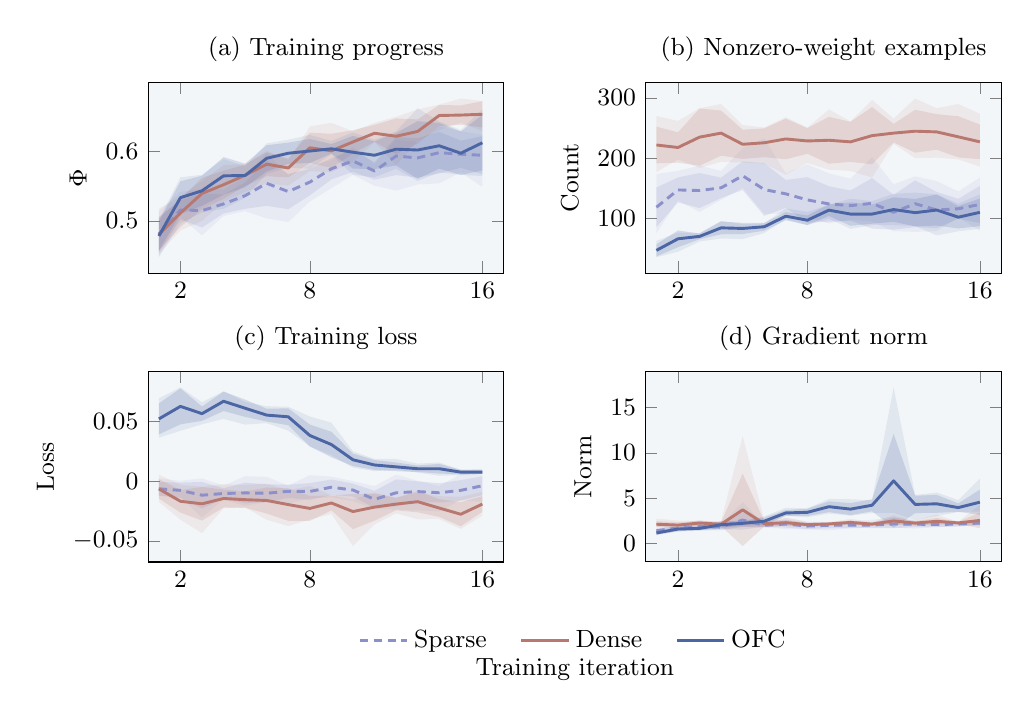
\begin{tikzpicture}\begin{groupplot}[group style={group size=2 by 2,horizontal sep=1.8cm,vertical sep=1.25cm},width=6.1cm,height=4.0cm,xmin=0.5,xmax=17.0,xtick={2,8,16},xlabel={Training iteration},axis background/.style={fill=diagramlight},tick label style={font=\footnotesize},title style={font=\small,yshift=-2pt},label style={font=\footnotesize},every axis plot/.append style={line join=round},tick label style={font=\small},label style={font=\small},legend style={font=\small,draw=none,fill=none,/tikz/every even column/.append style={column sep=1em}},legend columns=3]
\nextgroupplot[title={(a) Training progress},ylabel={$\Phi$},xlabel={}]
\addplot[name path=sparseaux0mma,draw=none,forget plot] coordinates {(1.00000,0.44965) (2.00000,0.50521) (3.00000,0.47917) (4.00000,0.50694) (5.00000,0.51389) (6.00000,0.50347) (7.00000,0.49826) (8.00000,0.52778) (9.00000,0.54688) (10.00000,0.56597) (11.00000,0.55035) (12.00000,0.54340) (13.00000,0.55208) (14.00000,0.55382) (15.00000,0.56944) (16.00000,0.54861)};
\addplot[name path=sparseaux0mmb,draw=none,forget plot] coordinates {(1.00000,0.51389) (2.00000,0.54167) (3.00000,0.54514) (4.00000,0.54514) (5.00000,0.56250) (6.00000,0.59722) (7.00000,0.56597) (8.00000,0.57986) (9.00000,0.58681) (10.00000,0.60590) (11.00000,0.58160) (12.00000,0.61632) (13.00000,0.61285) (14.00000,0.63542) (15.00000,0.62847) (16.00000,0.62326)};
\addplot[fill=sparsecolor,fill opacity=0.1,draw=none,forget plot] fill between[of=sparseaux0mma and sparseaux0mmb];
\addplot[name path=sparseaux0sda,draw=none,forget plot] coordinates {(1.00000,0.45579) (2.00000,0.50213) (3.00000,0.49043) (4.00000,0.51081) (5.00000,0.51730) (6.00000,0.52147) (7.00000,0.51679) (8.00000,0.53657) (9.00000,0.55940) (10.00000,0.57030) (11.00000,0.55903) (12.00000,0.56561) (13.00000,0.56207) (14.00000,0.56800) (15.00000,0.57603) (16.00000,0.56689)};
\addplot[name path=sparseaux0sdb,draw=none,forget plot] coordinates {(1.00000,0.50601) (2.00000,0.52912) (3.00000,0.53908) (4.00000,0.53780) (5.00000,0.55504) (6.00000,0.58617) (7.00000,0.56712) (8.00000,0.57454) (9.00000,0.58991) (10.00000,0.60157) (11.00000,0.58391) (12.00000,0.62015) (13.00000,0.61849) (14.00000,0.62760) (15.00000,0.61494) (16.00000,0.62119)};
\addplot[fill=sparsecolor,fill opacity=0.18,draw=none,forget plot] fill between[of=sparseaux0sda and sparseaux0sdb];
\addplot[sparsecolor,line width=1.05pt,mark=none,mark size=1.6pt,mark options={solid},densely dashed] coordinates {(1.00000,0.48090) (2.00000,0.51562) (3.00000,0.51476) (4.00000,0.52431) (5.00000,0.53617) (6.00000,0.55382) (7.00000,0.54196) (8.00000,0.55556) (9.00000,0.57465) (10.00000,0.58594) (11.00000,0.57147) (12.00000,0.59288) (13.00000,0.59028) (14.00000,0.59780) (15.00000,0.59549) (16.00000,0.59404)};
\addplot[name path=denseaux0mma,draw=none,forget plot] coordinates {(1.00000,0.45312) (2.00000,0.48611) (3.00000,0.50000) (4.00000,0.52778) (5.00000,0.54167) (6.00000,0.55382) (7.00000,0.55035) (8.00000,0.57118) (9.00000,0.56944) (10.00000,0.58507) (11.00000,0.61285) (12.00000,0.57986) (13.00000,0.61458) (14.00000,0.63021) (15.00000,0.64062) (16.00000,0.62847)};
\addplot[name path=denseaux0mmb,draw=none,forget plot] coordinates {(1.00000,0.51736) (2.00000,0.53472) (3.00000,0.55729) (4.00000,0.57986) (5.00000,0.58160) (6.00000,0.60069) (7.00000,0.58681) (8.00000,0.63542) (9.00000,0.64062) (10.00000,0.62847) (11.00000,0.64062) (12.00000,0.64931) (13.00000,0.65972) (14.00000,0.66667) (15.00000,0.67535) (16.00000,0.67188)};
\addplot[fill=densecolor,fill opacity=0.1,draw=none,forget plot] fill between[of=denseaux0mma and denseaux0mmb];
\addplot[name path=denseaux0sda,draw=none,forget plot] coordinates {(1.00000,0.45713) (2.00000,0.49138) (3.00000,0.51694) (4.00000,0.53157) (5.00000,0.55031) (6.00000,0.56411) (7.00000,0.56229) (8.00000,0.58299) (9.00000,0.57597) (10.00000,0.59643) (11.00000,0.61347) (12.00000,0.59564) (13.00000,0.61095) (14.00000,0.63603) (15.00000,0.63779) (16.00000,0.63398)};
\addplot[name path=denseaux0sdb,draw=none,forget plot] coordinates {(1.00000,0.50410) (2.00000,0.53119) (3.00000,0.56177) (4.00000,0.57202) (5.00000,0.58048) (6.00000,0.59851) (7.00000,0.58933) (8.00000,0.62650) (9.00000,0.62484) (10.00000,0.62984) (11.00000,0.63769) (12.00000,0.64683) (13.00000,0.64542) (14.00000,0.66606) (15.00000,0.66545) (16.00000,0.67157)};
\addplot[fill=densecolor,fill opacity=0.18,draw=none,forget plot] fill between[of=denseaux0sda and denseaux0sdb];
\addplot[densecolor,line width=1.05pt,mark=none,mark size=1.6pt,mark options={solid}] coordinates {(1.00000,0.48061) (2.00000,0.51128) (3.00000,0.53935) (4.00000,0.55179) (5.00000,0.56539) (6.00000,0.58131) (7.00000,0.57581) (8.00000,0.60475) (9.00000,0.60040) (10.00000,0.61314) (11.00000,0.62558) (12.00000,0.62124) (13.00000,0.62818) (14.00000,0.65104) (15.00000,0.65162) (16.00000,0.65278)};
\addplot[name path=sftaux0mma,draw=none,forget plot] coordinates {(1.00000,0.44792) (2.00000,0.49653) (3.00000,0.51215) (4.00000,0.51736) (5.00000,0.53299) (6.00000,0.56771) (7.00000,0.57639) (8.00000,0.57465) (9.00000,0.59549) (10.00000,0.56597) (11.00000,0.56250) (12.00000,0.57465) (13.00000,0.55729) (14.00000,0.56944) (15.00000,0.56597) (16.00000,0.56424)};
\addplot[name path=sftaux0mmb,draw=none,forget plot] coordinates {(1.00000,0.50174) (2.00000,0.56250) (3.00000,0.56597) (4.00000,0.58854) (5.00000,0.57812) (6.00000,0.61111) (7.00000,0.61632) (8.00000,0.62326) (9.00000,0.61458) (10.00000,0.62674) (11.00000,0.61632) (12.00000,0.62847) (13.00000,0.66146) (14.00000,0.64236) (15.00000,0.63021) (16.00000,0.65972)};
\addplot[fill=ofccolor,fill opacity=0.1,draw=none,forget plot] fill between[of=sftaux0mma and sftaux0mmb];
\addplot[name path=sftaux0sda,draw=none,forget plot] coordinates {(1.00000,0.45782) (2.00000,0.50984) (3.00000,0.52150) (4.00000,0.53764) (5.00000,0.54821) (6.00000,0.57098) (7.00000,0.58174) (8.00000,0.58298) (9.00000,0.59646) (10.00000,0.57494) (11.00000,0.57417) (12.00000,0.57939) (13.00000,0.56031) (14.00000,0.57485) (15.00000,0.56593) (16.00000,0.57223)};
\addplot[name path=sftaux0sdb,draw=none,forget plot] coordinates {(1.00000,0.49877) (2.00000,0.55671) (3.00000,0.56473) (4.00000,0.59141) (5.00000,0.58200) (6.00000,0.60842) (7.00000,0.61212) (8.00000,0.61726) (9.00000,0.61013) (10.00000,0.62182) (11.00000,0.61391) (12.00000,0.62605) (13.00000,0.64282) (14.00000,0.64043) (15.00000,0.62794) (16.00000,0.65173)};
\addplot[fill=ofccolor,fill opacity=0.18,draw=none,forget plot] fill between[of=sftaux0sda and sftaux0sdb];
\addplot[ofccolor,line width=1.05pt,mark=none,mark size=1.6pt,mark options={solid}] coordinates {(1.00000,0.47830) (2.00000,0.53328) (3.00000,0.54311) (4.00000,0.56453) (5.00000,0.56510) (6.00000,0.58970) (7.00000,0.59693) (8.00000,0.60012) (9.00000,0.60330) (10.00000,0.59838) (11.00000,0.59404) (12.00000,0.60272) (13.00000,0.60156) (14.00000,0.60764) (15.00000,0.59693) (16.00000,0.61198)};
\nextgroupplot[title={(b) Nonzero-weight examples},ylabel={Count},xlabel={}]
\addplot[name path=sparseaux1mma,draw=none,forget plot] coordinates {(1.00000,76.00000) (2.00000,130.00000) (3.00000,111.00000) (4.00000,131.00000) (5.00000,151.00000) (6.00000,108.00000) (7.00000,108.00000) (8.00000,101.00000) (9.00000,92.00000) (10.00000,98.00000) (11.00000,95.00000) (12.00000,79.00000) (13.00000,78.00000) (14.00000,79.00000) (15.00000,102.00000) (16.00000,80.00000)};
\addplot[name path=sparseaux1mmb,draw=none,forget plot] coordinates {(1.00000,174.00000) (2.00000,179.00000) (3.00000,188.00000) (4.00000,179.00000) (5.00000,217.00000) (6.00000,233.00000) (7.00000,175.00000) (8.00000,190.00000) (9.00000,175.00000) (10.00000,166.00000) (11.00000,202.00000) (12.00000,157.00000) (13.00000,170.00000) (14.00000,162.00000) (15.00000,145.00000) (16.00000,168.00000)};
\addplot[fill=sparsecolor,fill opacity=0.1,draw=none,forget plot] fill between[of=sparseaux1mma and sparseaux1mmb];
\addplot[name path=sparseaux1sda,draw=none,forget plot] coordinates {(1.00000,86.12605) (2.00000,126.76597) (3.00000,117.49828) (4.00000,134.11213) (5.00000,147.34413) (6.00000,104.46121) (7.00000,118.01305) (8.00000,93.32242) (9.00000,94.94853) (10.00000,96.49800) (11.00000,83.49714) (12.00000,81.67119) (13.00000,85.93855) (14.00000,84.17056) (15.00000,99.88138) (16.00000,92.73151)};
\addplot[name path=sparseaux1sdb,draw=none,forget plot] coordinates {(1.00000,151.54062) (2.00000,168.23403) (3.00000,175.50172) (4.00000,167.88787) (5.00000,194.65587) (6.00000,191.87212) (7.00000,163.98695) (8.00000,168.67758) (9.00000,153.71814) (10.00000,146.50200) (11.00000,167.16952) (12.00000,139.32881) (13.00000,163.39478) (14.00000,144.16278) (15.00000,132.78528) (16.00000,154.26849)};
\addplot[fill=sparsecolor,fill opacity=0.18,draw=none,forget plot] fill between[of=sparseaux1sda and sparseaux1sdb];
\addplot[sparsecolor,line width=1.05pt,mark=none,mark size=1.6pt,mark options={solid},densely dashed] coordinates {(1.00000,118.83333) (2.00000,147.50000) (3.00000,146.50000) (4.00000,151.00000) (5.00000,171.00000) (6.00000,148.16667) (7.00000,141.00000) (8.00000,131.00000) (9.00000,124.33333) (10.00000,121.50000) (11.00000,125.33333) (12.00000,110.50000) (13.00000,124.66667) (14.00000,114.16667) (15.00000,116.33333) (16.00000,123.50000)};
\addplot[name path=denseaux1mma,draw=none,forget plot] coordinates {(1.00000,177.00000) (2.00000,198.00000) (3.00000,184.00000) (4.00000,194.00000) (5.00000,193.00000) (6.00000,191.00000) (7.00000,173.00000) (8.00000,192.00000) (9.00000,181.00000) (10.00000,179.00000) (11.00000,168.00000) (12.00000,224.00000) (13.00000,200.00000) (14.00000,201.00000) (15.00000,198.00000) (16.00000,186.00000)};
\addplot[name path=denseaux1mmb,draw=none,forget plot] coordinates {(1.00000,270.00000) (2.00000,262.00000) (3.00000,283.00000) (4.00000,290.00000) (5.00000,255.00000) (6.00000,251.00000) (7.00000,268.00000) (8.00000,251.00000) (9.00000,281.00000) (10.00000,261.00000) (11.00000,297.00000) (12.00000,266.00000) (13.00000,299.00000) (14.00000,283.00000) (15.00000,290.00000) (16.00000,274.00000)};
\addplot[fill=densecolor,fill opacity=0.1,draw=none,forget plot] fill between[of=denseaux1mma and denseaux1mmb];
\addplot[name path=denseaux1sda,draw=none,forget plot] coordinates {(1.00000,191.57633) (2.00000,192.67450) (3.00000,187.52369) (4.00000,204.26257) (5.00000,198.98885) (6.00000,201.78641) (7.00000,198.31321) (8.00000,207.40010) (9.00000,191.00851) (10.00000,193.94368) (11.00000,189.98684) (12.00000,226.23078) (13.00000,209.27821) (14.00000,214.20030) (15.00000,201.46032) (16.00000,198.35405)};
\addplot[name path=denseaux1sdb,draw=none,forget plot] coordinates {(1.00000,252.42367) (2.00000,242.99216) (3.00000,282.47631) (4.00000,279.07077) (5.00000,247.34448) (6.00000,249.54692) (7.00000,265.68679) (8.00000,249.93323) (9.00000,268.65815) (10.00000,260.38965) (11.00000,285.01316) (12.00000,257.10256) (13.00000,280.38845) (14.00000,273.13303) (15.00000,269.53968) (16.00000,255.97928)};
\addplot[fill=densecolor,fill opacity=0.18,draw=none,forget plot] fill between[of=denseaux1sda and denseaux1sdb];
\addplot[densecolor,line width=1.05pt,mark=none,mark size=1.6pt,mark options={solid}] coordinates {(1.00000,222.00000) (2.00000,217.83333) (3.00000,235.00000) (4.00000,241.66667) (5.00000,223.16667) (6.00000,225.66667) (7.00000,232.00000) (8.00000,228.66667) (9.00000,229.83333) (10.00000,227.16667) (11.00000,237.50000) (12.00000,241.66667) (13.00000,244.83333) (14.00000,243.66667) (15.00000,235.50000) (16.00000,227.16667)};
\addplot[name path=sftaux1mma,draw=none,forget plot] coordinates {(1.00000,36.00000) (2.00000,45.00000) (3.00000,62.00000) (4.00000,67.00000) (5.00000,66.00000) (6.00000,76.00000) (7.00000,99.00000) (8.00000,89.00000) (9.00000,100.00000) (10.00000,83.00000) (11.00000,89.00000) (12.00000,89.00000) (13.00000,88.00000) (14.00000,72.00000) (15.00000,79.00000) (16.00000,83.00000)};
\addplot[name path=sftaux1mmb,draw=none,forget plot] coordinates {(1.00000,63.00000) (2.00000,77.00000) (3.00000,76.00000) (4.00000,96.00000) (5.00000,91.00000) (6.00000,92.00000) (7.00000,117.00000) (8.00000,111.00000) (9.00000,123.00000) (10.00000,133.00000) (11.00000,129.00000) (12.00000,141.00000) (13.00000,143.00000) (14.00000,140.00000) (15.00000,125.00000) (16.00000,140.00000)};
\addplot[fill=ofccolor,fill opacity=0.1,draw=none,forget plot] fill between[of=sftaux1mma and sftaux1mmb];
\addplot[name path=sftaux1sda,draw=none,forget plot] coordinates {(1.00000,37.36004) (2.00000,52.66165) (3.00000,65.73555) (4.00000,74.01459) (5.00000,74.37868) (6.00000,80.02698) (7.00000,97.30672) (8.00000,89.51882) (9.00000,104.40834) (10.00000,88.10155) (11.00000,91.54068) (12.00000,94.69237) (13.00000,87.06127) (14.00000,88.47296) (15.00000,83.70361) (16.00000,87.51521)};
\addplot[name path=sftaux1sdb,draw=none,forget plot] coordinates {(1.00000,57.30663) (2.00000,80.33835) (3.00000,75.26445) (4.00000,95.31874) (5.00000,92.95465) (6.00000,92.97302) (7.00000,110.69328) (8.00000,105.14785) (9.00000,123.59166) (10.00000,126.89845) (11.00000,123.45932) (12.00000,135.30763) (13.00000,132.60539) (14.00000,139.86038) (15.00000,120.96306) (16.00000,133.15145)};
\addplot[fill=ofccolor,fill opacity=0.18,draw=none,forget plot] fill between[of=sftaux1sda and sftaux1sdb];
\addplot[ofccolor,line width=1.05pt,mark=none,mark size=1.6pt,mark options={solid}] coordinates {(1.00000,47.33333) (2.00000,66.50000) (3.00000,70.50000) (4.00000,84.66667) (5.00000,83.66667) (6.00000,86.50000) (7.00000,104.00000) (8.00000,97.33333) (9.00000,114.00000) (10.00000,107.50000) (11.00000,107.50000) (12.00000,115.00000) (13.00000,109.83333) (14.00000,114.16667) (15.00000,102.33333) (16.00000,110.33333)};
\nextgroupplot[title={(c) Training loss},ylabel={Loss},xlabel={},scaled y ticks=false,yticklabel style={/pgf/number format/fixed,/pgf/number format/precision=2}]
\addplot[name path=sparseaux2mma,draw=none,forget plot] coordinates {(1.00000,-0.01208) (2.00000,-0.01353) (3.00000,-0.03054) (4.00000,-0.01530) (5.00000,-0.02068) (6.00000,-0.01736) (7.00000,-0.01870) (8.00000,-0.01444) (9.00000,-0.01353) (10.00000,-0.01667) (11.00000,-0.02336) (12.00000,-0.02383) (13.00000,-0.02444) (14.00000,-0.02521) (15.00000,-0.01592) (16.00000,-0.01748)};
\addplot[name path=sparseaux2mmb,draw=none,forget plot] coordinates {(1.00000,0.00203) (2.00000,0.00028) (3.00000,0.00221) (4.00000,-0.00373) (5.00000,0.00411) (6.00000,0.00346) (7.00000,-0.00365) (8.00000,0.00493) (9.00000,0.00378) (10.00000,-0.00002) (11.00000,-0.00412) (12.00000,0.00550) (13.00000,0.00031) (14.00000,-0.00416) (15.00000,0.00584) (16.00000,0.00547)};
\addplot[fill=sparsecolor,fill opacity=0.1,draw=none,forget plot] fill between[of=sparseaux2mma and sparseaux2mmb];
\addplot[name path=sparseaux2sda,draw=none,forget plot] coordinates {(1.00000,-0.01214) (2.00000,-0.01423) (3.00000,-0.02285) (4.00000,-0.01477) (5.00000,-0.01843) (6.00000,-0.01759) (7.00000,-0.01410) (8.00000,-0.01567) (9.00000,-0.01154) (10.00000,-0.01287) (11.00000,-0.02240) (12.00000,-0.02103) (13.00000,-0.01732) (14.00000,-0.01773) (15.00000,-0.01625) (16.00000,-0.01168)};
\addplot[name path=sparseaux2sdb,draw=none,forget plot] coordinates {(1.00000,-0.00076) (2.00000,-0.00127) (3.00000,-0.00074) (4.00000,-0.00599) (5.00000,-0.00133) (6.00000,-0.00270) (7.00000,-0.00302) (8.00000,-0.00167) (9.00000,0.00132) (10.00000,-0.00208) (11.00000,-0.00817) (12.00000,0.00144) (13.00000,-0.00022) (14.00000,-0.00179) (15.00000,0.00078) (16.00000,0.00396)};
\addplot[fill=sparsecolor,fill opacity=0.18,draw=none,forget plot] fill between[of=sparseaux2sda and sparseaux2sdb];
\addplot[sparsecolor,line width=1.05pt,mark=none,mark size=1.6pt,mark options={solid},densely dashed] coordinates {(1.00000,-0.00645) (2.00000,-0.00775) (3.00000,-0.01180) (4.00000,-0.01038) (5.00000,-0.00988) (6.00000,-0.01014) (7.00000,-0.00856) (8.00000,-0.00867) (9.00000,-0.00511) (10.00000,-0.00747) (11.00000,-0.01528) (12.00000,-0.00980) (13.00000,-0.00877) (14.00000,-0.00976) (15.00000,-0.00774) (16.00000,-0.00386)};
\addplot[name path=denseaux2mma,draw=none,forget plot] coordinates {(1.00000,-0.01745) (2.00000,-0.03226) (3.00000,-0.04356) (4.00000,-0.02275) (5.00000,-0.02191) (6.00000,-0.03233) (7.00000,-0.03757) (8.00000,-0.03211) (9.00000,-0.02761) (10.00000,-0.05428) (11.00000,-0.03618) (12.00000,-0.02698) (13.00000,-0.03194) (14.00000,-0.03180) (15.00000,-0.03996) (16.00000,-0.02898)};
\addplot[name path=denseaux2mmb,draw=none,forget plot] coordinates {(1.00000,0.00543) (2.00000,-0.00313) (3.00000,-0.00471) (4.00000,-0.00258) (5.00000,-0.00329) (6.00000,-0.00213) (7.00000,-0.00761) (8.00000,-0.00411) (9.00000,-0.01175) (10.00000,-0.01544) (11.00000,-0.00961) (12.00000,-0.01380) (13.00000,-0.00977) (14.00000,-0.01259) (15.00000,-0.01310) (16.00000,-0.00911)};
\addplot[fill=densecolor,fill opacity=0.1,draw=none,forget plot] fill between[of=denseaux2mma and denseaux2mmb];
\addplot[name path=denseaux2sda,draw=none,forget plot] coordinates {(1.00000,-0.01458) (2.00000,-0.02632) (3.00000,-0.03301) (4.00000,-0.02201) (5.00000,-0.02236) (6.00000,-0.02708) (7.00000,-0.03326) (8.00000,-0.03327) (9.00000,-0.02447) (10.00000,-0.04019) (11.00000,-0.03302) (12.00000,-0.02437) (13.00000,-0.02612) (14.00000,-0.02994) (15.00000,-0.03779) (16.00000,-0.02574)};
\addplot[name path=denseaux2sdb,draw=none,forget plot] coordinates {(1.00000,0.00152) (2.00000,-0.00745) (3.00000,-0.00496) (4.00000,-0.00707) (5.00000,-0.00869) (6.00000,-0.00531) (7.00000,-0.00600) (8.00000,-0.01239) (9.00000,-0.01211) (10.00000,-0.01071) (11.00000,-0.01044) (12.00000,-0.01407) (13.00000,-0.00830) (14.00000,-0.01511) (15.00000,-0.01758) (16.00000,-0.01266)};
\addplot[fill=densecolor,fill opacity=0.18,draw=none,forget plot] fill between[of=denseaux2sda and denseaux2sdb];
\addplot[densecolor,line width=1.05pt,mark=none,mark size=1.6pt,mark options={solid}] coordinates {(1.00000,-0.00653) (2.00000,-0.01688) (3.00000,-0.01898) (4.00000,-0.01454) (5.00000,-0.01553) (6.00000,-0.01620) (7.00000,-0.01963) (8.00000,-0.02283) (9.00000,-0.01829) (10.00000,-0.02545) (11.00000,-0.02173) (12.00000,-0.01922) (13.00000,-0.01721) (14.00000,-0.02252) (15.00000,-0.02769) (16.00000,-0.01920)};
\addplot[name path=sftaux2mma,draw=none,forget plot] coordinates {(1.00000,0.03633) (2.00000,0.04199) (3.00000,0.04737) (4.00000,0.05194) (5.00000,0.04715) (6.00000,0.04838) (7.00000,0.04208) (8.00000,0.02891) (9.00000,0.02153) (10.00000,0.01126) (11.00000,0.00829) (12.00000,0.00940) (13.00000,0.00704) (14.00000,0.00443) (15.00000,0.00496) (16.00000,0.00572)};
\addplot[name path=sftaux2mmb,draw=none,forget plot] coordinates {(1.00000,0.06919) (2.00000,0.07824) (3.00000,0.06584) (4.00000,0.07488) (5.00000,0.06622) (6.00000,0.06256) (7.00000,0.06203) (8.00000,0.05396) (9.00000,0.04879) (10.00000,0.02486) (11.00000,0.01846) (12.00000,0.01844) (13.00000,0.01457) (14.00000,0.01555) (15.00000,0.00946) (16.00000,0.01026)};
\addplot[fill=ofccolor,fill opacity=0.1,draw=none,forget plot] fill between[of=sftaux2mma and sftaux2mmb];
\addplot[name path=sftaux2sda,draw=none,forget plot] coordinates {(1.00000,0.03899) (2.00000,0.04736) (3.00000,0.05034) (4.00000,0.05851) (5.00000,0.05362) (6.00000,0.04975) (7.00000,0.04662) (8.00000,0.02893) (9.00000,0.01984) (10.00000,0.01259) (11.00000,0.00931) (12.00000,0.00824) (13.00000,0.00759) (14.00000,0.00633) (15.00000,0.00559) (16.00000,0.00600)};
\addplot[name path=sftaux2sdb,draw=none,forget plot] coordinates {(1.00000,0.06484) (2.00000,0.07741) (3.00000,0.06226) (4.00000,0.07479) (5.00000,0.06803) (6.00000,0.06041) (7.00000,0.06074) (8.00000,0.04722) (9.00000,0.04117) (10.00000,0.02299) (11.00000,0.01756) (12.00000,0.01552) (13.00000,0.01298) (14.00000,0.01432) (15.00000,0.00935) (16.00000,0.00902)};
\addplot[fill=ofccolor,fill opacity=0.18,draw=none,forget plot] fill between[of=sftaux2sda and sftaux2sdb];
\addplot[ofccolor,line width=1.05pt,mark=none,mark size=1.6pt,mark options={solid}] coordinates {(1.00000,0.05192) (2.00000,0.06239) (3.00000,0.05630) (4.00000,0.06665) (5.00000,0.06083) (6.00000,0.05508) (7.00000,0.05368) (8.00000,0.03808) (9.00000,0.03050) (10.00000,0.01779) (11.00000,0.01343) (12.00000,0.01188) (13.00000,0.01029) (14.00000,0.01032) (15.00000,0.00747) (16.00000,0.00751)};
\nextgroupplot[title={(d) Gradient norm},ylabel={Norm},xlabel={},legend to name=auxleg]
\addplot[name path=sparseaux3mma,draw=none,forget plot] coordinates {(1.00000,1.12500) (2.00000,1.39844) (3.00000,1.49219) (4.00000,1.53125) (5.00000,1.82031) (6.00000,1.75000) (7.00000,1.57031) (8.00000,1.51562) (9.00000,1.44531) (10.00000,1.62500) (11.00000,1.74219) (12.00000,1.74219) (13.00000,1.61719) (14.00000,1.80469) (15.00000,1.82812) (16.00000,2.03125)};
\addplot[name path=sparseaux3mmb,draw=none,forget plot] coordinates {(1.00000,1.65625) (2.00000,2.07812) (3.00000,2.56250) (4.00000,2.09375) (5.00000,4.53125) (6.00000,2.10938) (7.00000,2.79688) (8.00000,2.40625) (9.00000,2.40625) (10.00000,2.42188) (11.00000,2.59375) (12.00000,2.92188) (13.00000,2.46875) (14.00000,2.48438) (15.00000,2.37500) (16.00000,2.65625)};
\addplot[fill=sparsecolor,fill opacity=0.1,draw=none,forget plot] fill between[of=sparseaux3mma and sparseaux3mmb];
\addplot[name path=sparseaux3sda,draw=none,forget plot] coordinates {(1.00000,1.22855) (2.00000,1.46005) (3.00000,1.50041) (4.00000,1.56606) (5.00000,1.50668) (6.00000,1.84535) (7.00000,1.73073) (8.00000,1.57390) (9.00000,1.66324) (10.00000,1.71083) (11.00000,1.68212) (12.00000,1.66820) (13.00000,1.78684) (14.00000,1.77690) (15.00000,1.88851) (16.00000,1.99071)};
\addplot[name path=sparseaux3sdb,draw=none,forget plot] coordinates {(1.00000,1.57093) (2.00000,1.91495) (3.00000,2.25219) (4.00000,2.00686) (5.00000,3.62873) (6.00000,2.12861) (7.00000,2.53489) (8.00000,2.22819) (9.00000,2.30811) (10.00000,2.27875) (11.00000,2.35173) (12.00000,2.59743) (13.00000,2.43191) (14.00000,2.37154) (15.00000,2.35368) (16.00000,2.47804)};
\addplot[fill=sparsecolor,fill opacity=0.18,draw=none,forget plot] fill between[of=sparseaux3sda and sparseaux3sdb];
\addplot[sparsecolor,line width=1.05pt,mark=none,mark size=1.6pt,mark options={solid},densely dashed] coordinates {(1.00000,1.39974) (2.00000,1.68750) (3.00000,1.87630) (4.00000,1.78646) (5.00000,2.56771) (6.00000,1.98698) (7.00000,2.13281) (8.00000,1.90104) (9.00000,1.98568) (10.00000,1.99479) (11.00000,2.01693) (12.00000,2.13281) (13.00000,2.10938) (14.00000,2.07422) (15.00000,2.12109) (16.00000,2.23438)};
\addlegendentry{Sparse}
\addplot[name path=denseaux3mma,draw=none,forget plot] coordinates {(1.00000,1.82031) (2.00000,1.60938) (3.00000,1.80469) (4.00000,1.77344) (5.00000,1.82031) (6.00000,1.74219) (7.00000,1.94531) (8.00000,1.85156) (9.00000,1.93750) (10.00000,2.04688) (11.00000,1.94531) (12.00000,2.06250) (13.00000,1.93750) (14.00000,2.17188) (15.00000,2.04688) (16.00000,2.00000)};
\addplot[name path=denseaux3mmb,draw=none,forget plot] coordinates {(1.00000,2.73438) (2.00000,2.51562) (3.00000,2.46875) (4.00000,2.45312) (5.00000,11.87500) (6.00000,2.57812) (7.00000,2.85938) (8.00000,2.35938) (9.00000,2.29688) (10.00000,2.71875) (11.00000,2.35938) (12.00000,3.10938) (13.00000,2.53125) (14.00000,3.17188) (15.00000,2.39062) (16.00000,4.28125)};
\addplot[fill=densecolor,fill opacity=0.1,draw=none,forget plot] fill between[of=denseaux3mma and denseaux3mmb];
\addplot[name path=denseaux3sda,draw=none,forget plot] coordinates {(1.00000,1.76869) (2.00000,1.70142) (3.00000,1.98069) (4.00000,1.89235) (5.00000,-0.31063) (6.00000,1.85454) (7.00000,1.94796) (8.00000,1.88816) (9.00000,2.01286) (10.00000,2.05729) (11.00000,1.97423) (12.00000,2.07209) (13.00000,2.01868) (14.00000,2.05578) (15.00000,2.12229) (16.00000,1.65664)};
\addplot[name path=denseaux3sdb,draw=none,forget plot] coordinates {(1.00000,2.44225) (2.00000,2.32201) (3.00000,2.49587) (4.00000,2.32900) (5.00000,7.71427) (6.00000,2.45536) (7.00000,2.61193) (8.00000,2.23423) (9.00000,2.26318) (10.00000,2.55209) (11.00000,2.26275) (12.00000,2.87062) (13.00000,2.43965) (14.00000,2.80881) (15.00000,2.37771) (16.00000,3.40065)};
\addplot[fill=densecolor,fill opacity=0.18,draw=none,forget plot] fill between[of=denseaux3sda and denseaux3sdb];
\addplot[densecolor,line width=1.05pt,mark=none,mark size=1.6pt,mark options={solid}] coordinates {(1.00000,2.10547) (2.00000,2.01172) (3.00000,2.23828) (4.00000,2.11068) (5.00000,3.70182) (6.00000,2.15495) (7.00000,2.27995) (8.00000,2.06120) (9.00000,2.13802) (10.00000,2.30469) (11.00000,2.11849) (12.00000,2.47135) (13.00000,2.22917) (14.00000,2.43229) (15.00000,2.25000) (16.00000,2.52865)};
\addlegendentry{Dense}
\addplot[name path=sftaux3mma,draw=none,forget plot] coordinates {(1.00000,0.93750) (2.00000,1.28906) (3.00000,1.38281) (4.00000,1.44531) (5.00000,1.81250) (6.00000,1.84375) (7.00000,3.03125) (8.00000,2.87500) (9.00000,3.28125) (10.00000,3.04688) (11.00000,3.34375) (12.00000,3.35938) (13.00000,2.54688) (14.00000,3.01562) (15.00000,3.45312) (16.00000,3.51562)};
\addplot[name path=sftaux3mmb,draw=none,forget plot] coordinates {(1.00000,1.50781) (2.00000,1.82031) (3.00000,1.82031) (4.00000,2.46875) (5.00000,2.45312) (6.00000,2.98438) (7.00000,3.92188) (8.00000,3.85938) (9.00000,4.90625) (10.00000,4.87500) (11.00000,4.75000) (12.00000,17.25000) (13.00000,5.34375) (14.00000,5.62500) (15.00000,4.78125) (16.00000,7.15625)};
\addplot[fill=ofccolor,fill opacity=0.1,draw=none,forget plot] fill between[of=sftaux3mma and sftaux3mmb];
\addplot[name path=sftaux3sda,draw=none,forget plot] coordinates {(1.00000,0.92673) (2.00000,1.33809) (3.00000,1.45036) (4.00000,1.69394) (5.00000,1.96258) (6.00000,2.04919) (7.00000,3.04002) (8.00000,3.02070) (9.00000,3.45181) (10.00000,3.11357) (11.00000,3.53750) (12.00000,1.70721) (13.00000,3.33921) (14.00000,3.37254) (15.00000,3.47524) (16.00000,3.15774)};
\addplot[name path=sftaux3sdb,draw=none,forget plot] coordinates {(1.00000,1.35062) (2.00000,1.81034) (3.00000,1.84651) (4.00000,2.40763) (5.00000,2.44888) (6.00000,2.82581) (7.00000,3.67353) (8.00000,3.82305) (9.00000,4.64194) (10.00000,4.44372) (11.00000,4.87395) (12.00000,12.10529) (13.00000,5.25975) (14.00000,5.35663) (15.00000,4.41539) (16.00000,5.93601)};
\addplot[fill=ofccolor,fill opacity=0.18,draw=none,forget plot] fill between[of=sftaux3sda and sftaux3sdb];
\addplot[ofccolor,line width=1.05pt,mark=none,mark size=1.6pt,mark options={solid}] coordinates {(1.00000,1.13867) (2.00000,1.57422) (3.00000,1.64844) (4.00000,2.05078) (5.00000,2.20573) (6.00000,2.43750) (7.00000,3.35677) (8.00000,3.42188) (9.00000,4.04688) (10.00000,3.77865) (11.00000,4.20573) (12.00000,6.90625) (13.00000,4.29948) (14.00000,4.36458) (15.00000,3.94531) (16.00000,4.54688)};
\addlegendentry{OFC}
\end{groupplot}
\node[anchor=north] at ($(group c1r2.south)!0.5!(group c2r2.south)+(0,-0.6cm)$) {\pgfplotslegendfromname{auxleg}};
\node[anchor=north,font=\small] at ($(group c1r2.south)!0.5!(group c2r2.south)+(0,-1.1cm)$) {Training iteration};
\end{tikzpicture}
}
\end{document}
